\documentclass[11pt]{article}

\usepackage{amsmath,amssymb,amsthm,mathtools,bm}
\usepackage{booktabs}
\usepackage{geometry}
\usepackage{enumitem}
\usepackage{hyperref}
\usepackage{xcolor}
\usepackage{graphicx}

\geometry{margin=1in}

% ------------------------------------------------------------
% Draft status
% ------------------------------------------------------------
% Updated after the latest algorithmic development (2026-08-26).
% The main algorithmic line in this draft is now:
%   admissible convexity-preserving kinetic-term regularization
%   + vacuum-compatible potential regularization
%   + positivity/mass-preserving Fourier pseudospectral discretization
%   + FISTA-CD with potential-proximal splitting
%   + interior Newton-PCG stationarity refinement.
%
% Numerical tables remain placeholders unless a value has already been
% certified by the current code.  No unrun convergence claim is made.
% ------------------------------------------------------------

\newcommand{\R}{\mathbb{R}}
\newcommand{\C}{\mathbb{C}}
\newcommand{\A}{\mathcal{A}}
\newcommand{\E}{\mathcal{E}}
\newcommand{\CN}{\mathcal{C}_N}
\newcommand{\SN}{S_N}
\newcommand{\SNP}{S_N^+}
\newcommand{\PN}{P_N}
\newcommand{\dd}{\,\mathrm{d}}
\newcommand{\ii}{\mathrm{i}}
\newcommand{\eps}{\varepsilon}
\newcommand{\sig}{\sigma}
\newcommand{\inner}[2]{\left\langle #1,#2\right\rangle}
\newcommand{\norm}[1]{\left\|#1\right\|}
\newcommand{\abs}[1]{\left|#1\right|}
\newcommand{\grad}{\nabla}
\newcommand{\half}{\frac12}
\newcommand{\todo}[1]{\textcolor{red}{[TODO: #1]}}

\theoremstyle{plain}
\newtheorem{theorem}{Theorem}[section]
\newtheorem{lemma}[theorem]{Lemma}
\newtheorem{proposition}[theorem]{Proposition}
\newtheorem{corollary}[theorem]{Corollary}

\theoremstyle{definition}
\newtheorem{definition}[theorem]{Definition}
\newtheorem{remark}[theorem]{Remark}

\numberwithin{equation}{section}
\counterwithin{figure}{section}
\counterwithin{table}{section}

\title{\bf
A positive-conservative Fourier optimization method for ground states of Bose--Einstein condensates with higher-order interactions
}

\author{
Bo Lin\thanks{} \,  and 
Xinran Ruan\thanks{(Corresponding author) School of Mathematical Sciences, Capital Normal University, Beijing 100048, People's Republic of China {\tt (xinran.ruan@cnu.edu.cn)}.}
}
\date{}

\begin{document}
\maketitle

\begin{abstract}
We develop a positive-conservative Fourier optimization (PCFO) method for computing ground
states of Bose--Einstein condensates with higher-order interactions.
In the density formulation, the kinetic term is singular at vacuum.
We regularize this term through a positive concave denominator and
combine it with a compatible convex regularization of the potential to remove
its nonzero vacuum slope. The resulting energies preserve convexity,
and their fixed-box $\Gamma$-convergence to the original density energy is
established as the regularization parameters vanish. The Fourier
discretization preserves mass exactly and imposes positivity at the
collocation points.  
To avoid the large curvature introduced by the potential regularization, we
place this term together with the constraints in the proximal part of
an accelerated first-order method and use a Newton--PCG refinement for
high-accuracy stationarity. Numerical experiments demonstrate
spectral-type convergence for fixed smooth regularized problems,
examine the effects of the two regularization scales, and confirm the
efficiency of the two-stage optimization strategy.
\end{abstract}

\noindent
\textbf{Key words.}
Bose--Einstein condensate; higher-order interaction; density
formulation; convex optimization; Fourier
pseudospectral method; positivity preserving. 

\medskip

\noindent
\textbf{2020 MSC.}
35Q55, 65N35, 65K10, 90C25.


% ============================================================
\section{Introduction}
% ============================================================

Bose--Einstein condensation, first realized experimentally in dilute
atomic gases in 1995 \cite{Anderson1995}, provides a fundamental
setting for the study of macroscopic quantum phenomena. In the dilute
and low-temperature regime, Bose--Einstein condensates are commonly
described by the Gross--Pitaevskii equation \cite{BaoCaiReview}. With
tunable interactions, in particular near Feshbach resonances
\cite{Chin2010}, finite-range corrections to the standard contact
interaction may become relevant
\cite{FuWangGao2003,CollinMassignanPethick2007,
ZinnerThogersen2009,VekslerFishmanKetterle2014}. These corrections lead
to modified Gross--Pitaevskii models with higher-order interactions.

We consider the modified Gross--Pitaevskii model with higher-order
interactions (HOI), whose ground-state energy is
\begin{equation}
\label{eq:wave-energy}
E(\phi)
=
\int_{\R^d}
\left[
\half |\grad\phi|^2
+V(x)|\phi|^2
+\frac{\beta}{2}|\phi|^4
+\frac{\delta}{2}\bigl|\grad(|\phi|^2)\bigr|^2
\right]\dd x,
\end{equation}
subject to
\begin{equation}
\label{eq:wave-mass}
\norm{\phi}_{L^2}^2=1.
\end{equation}
Here $V\ge0$ is a confining potential, $\beta\in\R$ is the
contact-interaction strength, and $\delta>0$ is the higher-order
interaction strength. Ground-state properties and asymptotic regimes
for this model have been studied in
\cite{RuanCaiBao2016,BaoCaiRuan2019}. In this work, we focus on the
repulsive regime $\beta\ge0$.

A ground state may be chosen real and nonnegative. Introducing the
density $\rho=|\phi|^2$ then gives the equivalent energy
\begin{equation}
\label{eq:density-energy}
\E_0(\rho)
=
\int_{\R^d}
\left[
\frac{|\grad\rho|^2}{8\rho}
+V(x)\rho
+\frac{\beta}{2}\rho^2
+\frac{\delta}{2}|\grad\rho|^2
\right]\dd x,
\end{equation}
over
\begin{equation}
\label{eq:admissible-density}
\A
=
\left\{
\rho\in H^1(\R^d):
\rho\ge0,\quad
\int_{\R^d}\rho\,\dd x=1,\quad
\int_{\R^d}V\rho\,\dd x<\infty
\right\}.
\end{equation}
The singular kinetic term in \eqref{eq:density-energy} is understood
in the extended sense specified in Section~\ref{sec:density}.
For $\beta\ge0$, the density formulation has a convex structure that
is particularly attractive for ground-state computation, but the
kinetic term becomes singular at vacuum.

Ground-state computation for the Gross--Pitaevskii equation has been
studied extensively. Early approaches include direct energy
minimization and normalized gradient-flow methods
\cite{BaoTang2003,BaoDu2004}, together with spectrally accurate
discretizations \cite{BaoChernLim2006}. For strongly nonlinear or
rotating condensates, Sobolev-gradient methods, preconditioned
spectral solvers, nonlinear conjugate-gradient methods, regularized
Newton methods, and Riemannian optimization have been developed
\cite{DanailaKazemi2010,AntoineDuboscq2014,
AntoineLevittTang2017,WuWenBao2017,DanailaProtas2017}. More recent work
includes normalized Sobolev-gradient flows and nonlinear eigenvalue
iterations with convergence analysis
\cite{HenningPeterseim2020,AltmannHenningPeterseim2021,
ChenLuLuZhang2024}. Fourier pseudospectral discretizations combined
with manifold optimization have also been applied to more general
spinor condensates \cite{TianCaiWuWen2020}.

For the HOI model, a normalized gradient-flow method with an
attractive--repulsive splitting was developed in \cite{Ruan2018}.
W. Bao and X. Ruan \cite{BaoRuan2019} subsequently introduced a regularized
density formulation, in which the ground-state problem is treated as
a convex minimization problem using a shifted kinetic regularization,
a second-order finite-difference discretization, and an accelerated
projected-gradient method. A related square-root regularization of the
potential was also considered there as a numerical enhancement.

The present work builds on this density formulation with the aim of
achieving high spatial accuracy and high-accuracy stationarity.
Regularizing the kinetic term alone leaves a nonzero potential slope
at vacuum, which may produce an active positivity set and limit the
regularity seen by a Fourier discretization. Moreover, decreasing the
potential-regularization scale introduces large local curvature,
while the final stationarity can become difficult to resolve
efficiently by a first-order iteration alone.

To address these issues, we consider a general convexity-preserving
regularization of the kinetic denominator together with an
independently scaled convex regularization of the potential, and
establish the fixed-box $\Gamma$-convergence of the jointly regularized
energies. The resulting problem is discretized by a Fourier
pseudospectral method with exact mass conservation and nodal
positivity. A potential-proximal accelerated iteration is used for the
main minimization, followed by a Newton--PCG refinement for
high-accuracy stationarity. Numerical experiments examine spatial
accuracy, regularization effects, and solver performance, and
illustrate the method for two-dimensional trapping potentials.

The rest of the paper is organized as follows.
Section~\ref{sec:density} introduces the convex regularizations and
establishes their fixed-box variational convergence.
Section~\ref{sec:ps} presents the Fourier pseudospectral discretization
and the positive mass-conservative projection.
Section~\ref{sec:opt} develops the potential-proximal FISTA method and
the Newton--PCG refinement. Section~\ref{sec:num} reports the numerical
results, and Section~\ref{sec:summary} concludes the paper.

% ============================================================
\section{Density formulation and convex regularization}
\label{sec:density}
% ============================================================

In this section, we formulate the ground-state problem in terms of the
density and study convex regularizations of the singular kinetic term
and the potential term. We first describe the convex structure of the
density energy and construct the two regularizations. We then
establish their variational convergence on a fixed periodic box as the
regularization parameters vanish.


\subsection{Convex regularization of the kinetic and potential terms}

We first regularize the density kinetic term while preserving its
convex structure, and then combine it with a compatible regularization
of the potential term near vacuum.

\paragraph{Kinetic regularization.}

We begin by extending the density kinetic term to possible vacuum
regions.
For $s\ge0$ and $q\in\R^d$, let
\begin{equation}
\label{eq:kinetic-integrand}
F_0(s,q)
=
\begin{cases}
\dfrac{|q|^2}{8s}, & s>0,\\[1ex]
0, & s=0,\ q=0,\\
+\infty, & s=0,\ q\ne0.
\end{cases}
\end{equation}
With this convention, the density energy in
\eqref{eq:density-energy} can be written as
\begin{equation}
\label{eq:density-energy-extended}
\E_0(\rho)
=
\int_{\R^d}
\left[
F_0(\rho,\nabla\rho)
+V\rho
+\frac{\beta}{2}\rho^2
+\frac{\delta}{2}|\nabla\rho|^2
\right]\dd x,
\qquad
\rho\in\A.
\end{equation}

We first record the convexity property that motivates the
regularization introduced below.

\begin{proposition}[Convexity of the density energy]
\label{prop:density-convexity}
Assume $\beta\ge0$ and $\delta>0$.
Then $\E_0$ is strictly convex on $\A$ and hence has at most one
minimizer.
\end{proposition}

\begin{proof}
The map $(s,q)\mapsto |q|^2/s$ is the perspective of the convex
quadratic function $q\mapsto |q|^2$, and
\eqref{eq:kinetic-integrand} is its lower-semicontinuous convex
extension to $s=0$. The potential term is linear, while the remaining
terms are convex.

The term
$\frac{\delta}{2}\|\nabla\rho\|_{L^2}^2$
provides strict convexity. Indeed, equality in its convexity
inequality for two densities in $\A$ implies that their gradients
coincide almost everywhere. Their difference is therefore constant.
Since both densities are integrable on $\R^d$, this constant must be
zero.
\end{proof}

We now regularize the kinetic term in a way that preserves this
convexity. For $s\ge0$ and $q\in\R^d$, set
\begin{equation}
\label{eq:regularized-kinetic-integrand}
F_\eps(s,q)
=
\frac{|q|^2}{8r_\eps(s)},
\end{equation}
where $r_\eps$ is a positive regularization of the denominator.

\begin{definition}[Admissible denominator]
\label{def:admissible-regularization}
A family $\{r_\eps\}_{\eps>0}$ is called admissible if, for every
$\eps>0$,
\begin{equation}
\label{eq:regularization-admissibility-local}
r_\eps\in C^1([0,\infty)),
\qquad
r_\eps>0,
\qquad
r_\eps'\ge0,
\qquad
r_\eps \text{ is concave},
\end{equation}
and, for every $s\ge0$,
\begin{equation}
\label{eq:regularization-admissibility-limit}
s
\le
r_{\eps_1}(s)
\le
r_{\eps_2}(s)
\quad
\text{for }0<\eps_1\le\eps_2,
\qquad
r_\eps(s)\to s
\quad\text{as }\eps\to0^+.
\end{equation}
\end{definition}

The concavity of the denominator is precisely what preserves the
convexity of the regularized kinetic term.

\begin{lemma}[Convexity of the regularized kinetic integrand]
\label{lem:regularized-kinetic-convexity}
Let $r_\eps$ be admissible in the sense of Definition \ref{def:admissible-regularization}. Then
\[
F_\eps(s,q)
=
\frac{|q|^2}{8r_\eps(s)}
\]
is jointly convex in $(s,q)\in[0,\infty)\times\R^d$.
\end{lemma}

\begin{proof}
Let $0\le\theta\le1$ and set
\[
s_\theta=\theta s_1+(1-\theta)s_2,
\qquad
q_\theta=\theta q_1+(1-\theta)q_2.
\]
By the concavity of $r_\eps$,
\[
r_\eps(s_\theta)
\ge
\theta r_\eps(s_1)+(1-\theta)r_\eps(s_2).
\]
Hence
\[
F_\eps(s_\theta,q_\theta)
\le
\frac{|q_\theta|^2}
{8[\theta r_\eps(s_1)+(1-\theta)r_\eps(s_2)]}.
\]
The weighted Cauchy--Schwarz inequality gives
\[
\frac{|q_\theta|^2}
{\theta r_\eps(s_1)+(1-\theta)r_\eps(s_2)}
\le
\theta\frac{|q_1|^2}{r_\eps(s_1)}
+
(1-\theta)\frac{|q_2|^2}{r_\eps(s_2)},
\]
which proves the result.
\end{proof} 

The simplest example is the shifted denominator introduced in
\cite{BaoRuan2019},
\begin{equation}
\label{eq:shift-denominator}
r_\eps^{\rm sh}(s)=s+\eps.
\end{equation}
For comparison, we also consider the family
\begin{equation}
\label{eq:piecewise-regularization-family}
r_{\eps,m}(s)
=
\begin{cases}
s+\eps-\dfrac{\eps}{m+1}
\left(1-\dfrac{s}{\eps}\right)^{m+1},
&0\le s\le\eps,\\[2ex]
s+\eps,
&s>\eps,
\end{cases}
\qquad m=1,2.
\end{equation}
These functions belong to $C^m([0,\infty))$ and satisfy
Definition~\ref{def:admissible-regularization}. The cases $m=1,2$
are included in the numerical comparison below.

\paragraph{Potential regularization.}

The kinetic regularization removes the singularity at $\rho=0$, but
the linear potential term $V\rho$ still has the nonzero vacuum
derivative $V$. In the discrete problem this may produce an active
positivity set and thereby limit the attainable Fourier accuracy.
We therefore regularize the potential contribution near vacuum by
replacing $\rho$ with
\begin{equation}
\label{eq:potential-regularizer}
p_\sig(s)
=
\sqrt{s^2+\sig^2}-\sig,
\qquad s\ge0.
\end{equation}
A square-root smoothing of this type was already considered as a
numerical enhancement in \cite{BaoRuan2019}. Here $\sig$ is treated as
an independent regularization scale and the two regularizations are
analyzed jointly.
It satisfies
\begin{equation}
\label{eq:potential-regularizer-derivatives}
p_\sig(0)=p_\sig'(0)=0,
\qquad
p_\sig''(s)
=
\frac{\sig^2}{(s^2+\sig^2)^{3/2}}
\ge0.
\end{equation}
Hence $Vp_\sig$ is convex whenever $V\ge0$. Moreover,
$p_\sig(s)\to s$ as $\sig\to0^+$. For the convergence analysis below,
it is sufficient to assume that
$\sig=\sig(\eps)\to0$ as $\eps\to0^+$.

Combining the two regularizations, we obtain
\begin{equation}
\label{eq:joint-regularized-energy}
\E_{\eps,\sig}(\rho)
=
\int_{\R^d}
\left[
F_\eps(\rho,\nabla\rho)
+V(x)p_\sig(\rho)
+\frac{\beta}{2}\rho^2
+\frac{\delta}{2}|\nabla\rho|^2
\right]\dd x,
\qquad
\rho\in\A.
\end{equation}

The convex structure of the original density problem is retained by
the regularized energy.

\begin{proposition}[Convexity of the regularized energy]
\label{prop:joint-convexity}
Assume that $r_\eps$ is admissible in the sense of Definition \ref{def:admissible-regularization}, $V\ge0$, $\beta\ge0$,
$\delta>0$, and $\sig>0$.
Then $\E_{\eps,\sig}$ is strictly convex on $\A$.
If $\beta>0$, it is strongly convex with respect to the $L^2$ norm.
\end{proposition}

\begin{proof}
By Lemma~\ref{lem:regularized-kinetic-convexity}, the kinetic
contribution is convex. The potential term is convex because
$p_\sig$ is convex and $V\ge0$, while the remaining terms are convex.
Strict convexity follows from the $\delta$ term as in
Proposition~\ref{prop:density-convexity}. If $\beta>0$, the term
$\frac{\beta}{2}\|\rho\|_{L^2}^2$ gives strong convexity in $L^2$.
\end{proof}

The two properties of $p_\sig$ play different roles.
The condition $p_\sig'(0)=0$ removes the nonzero vacuum slope of the
potential term, while the curvature $p_\sig''(0)=1/\sig$ motivates
the proximal treatment introduced in Section~\ref{subsec:potential_FISTA}.


\subsection{Fixed-box $\Gamma$-convergence}

We next study the limit of the regularized problem as the
regularization parameters vanish. Since the Fourier discretization
considered below is posed on a periodic computational box, we carry
out the variational analysis for a fixed
$D_L=[-L,L)^d$. This separates the regularization limit from the
choice of computational box.
We use the standard notion of $\Gamma$-convergence in the strong
$L^2(D_L)$ topology; see, e.g., \cite{Braides2002}.

Define
\begin{equation}
\label{eq:admissible-density-box}
\A_L
=
\left\{
\rho\in H^1_{\rm per}(D_L):
\rho\ge0\ {\rm a.e.},
\quad
\int_{D_L}\rho\,\dd x=1
\right\}.
\end{equation}
The corresponding fixed-box energies are
\begin{equation}
\label{eq:fixed-box-energies}
\begin{aligned}
\E_{0,L}(\rho)
&=
\int_{D_L}
\left[
F_0(\rho,\nabla\rho)
+V\rho
+\frac{\beta}{2}\rho^2
+\frac{\delta}{2}|\nabla\rho|^2
\right]\dd x,\\
\E_{\eps,\sig,L}(\rho)
&=
\int_{D_L}
\left[
F_\eps(\rho,\nabla\rho)
+Vp_\sig(\rho)
+\frac{\beta}{2}\rho^2
+\frac{\delta}{2}|\nabla\rho|^2
\right]\dd x,
\qquad
\rho\in\A_L.
\end{aligned}
\end{equation}

The potential regularization introduces only a uniformly small
perturbation on a fixed box. Indeed, for every $s\ge0$,
\begin{equation}
\label{eq:potential-energy-defect}
0\le s-p_\sig(s)\le\sig,
\qquad
\left|
\int_{D_L}
V\,[p_\sig(\rho)-\rho]\,\dd x
\right|
\le
\sig\int_{D_L}V\,\dd x.
\end{equation}
This estimate allows the kinetic and potential regularizations to be
treated separately in the convergence argument.

\begin{theorem}[$\Gamma$-convergence of the joint regularization]
\label{thm:gamma-joint}
Let $V\in C(D_L)$ with $V\ge0$, $\beta\ge0$, and $\delta>0$.
Let $\{r_\eps\}$ be admissible in the sense of
Definition~\ref{def:admissible-regularization}, and let
$\sig(\eps)>0$ satisfy
$\sig(\eps)\to0$ as $\eps\to0^+$.
Extend $\E_{\eps,\sig(\eps),L}$ and $\E_{0,L}$ to $L^2(D_L)$
by setting them equal to $+\infty$ outside $\A_L$.
Then
\[
\E_{\eps,\sig(\eps),L}
\xrightarrow{\Gamma}
\E_{0,L}
\qquad
\text{in the strong }L^2(D_L)\text{ topology}.
\]
Moreover, the family
$\{\E_{\eps,\sig(\eps),L}\}_{\eps>0}$
is equicoercive in $L^2(D_L)$.
\end{theorem}

\begin{proof}
We first consider the kinetic regularization alone and keep the
potential term unchanged. Define
\[
\widetilde\E_{\eps,L}(\rho)
=
\int_{D_L}
\left[
F_\eps(\rho,\nabla\rho)
+V\rho
+\frac{\beta}{2}\rho^2
+\frac{\delta}{2}|\nabla\rho|^2
\right]\dd x.
\]

We first prove the liminf inequality. Let $\eps_n\to0$ and
$\rho_n\to\rho$ strongly in $L^2(D_L)$. If
\[
\liminf_{n\to\infty}
\widetilde\E_{\eps_n,L}(\rho_n)=+\infty,
\]
there is nothing to prove. Otherwise, after passing to a subsequence,
we may assume that the energies are uniformly bounded. Since
$\delta>0$, the gradient term together with the fixed mass gives a
uniform $H^1(D_L)$ bound. Hence, after extracting a further
subsequence,
\[
\rho_n\rightharpoonup\rho
\qquad
\text{weakly in }H^1(D_L).
\]

Fix $\bar\eps>0$. For all sufficiently large $n$,
$\eps_n\le\bar\eps$. The ordering in
\eqref{eq:regularization-admissibility-limit} therefore gives
\[
F_{\eps_n}(s,q)
\ge
F_{\bar\eps}(s,q).
\]
For fixed $\bar\eps$, the integrand $F_{\bar\eps}$ is continuous and
jointly convex in $(s,q)$. The associated integral functional is
therefore weakly lower semicontinuous on $H^1(D_L)$. Together with
the remaining terms, this yields
\[
\liminf_{n\to\infty}
\widetilde\E_{\eps_n,L}(\rho_n)
\ge
\widetilde\E_{\bar\eps,L}(\rho).
\]
Finally, let $\bar\eps\downarrow0$. Since
$r_{\bar\eps}(s)\downarrow s$, the nonnegative kinetic integrands
increase pointwise to $F_0$. The monotone convergence theorem then
gives
\[
\liminf_{n\to\infty}
\widetilde\E_{\eps_n,L}(\rho_n)
\ge
\E_{0,L}(\rho).
\]

For the recovery sequence, let $\rho\in\A_L$ satisfy
$\E_{0,L}(\rho)<\infty$ and take the constant sequence
$\rho_\eps=\rho$. The same monotone convergence argument gives
\[
\widetilde\E_{\eps,L}(\rho)
\longrightarrow
\E_{0,L}(\rho)
\qquad
\text{as }\eps\to0^+.
\]
Hence
\[
\widetilde\E_{\eps,L}
\xrightarrow{\Gamma}
\E_{0,L}
\qquad
\text{in strong }L^2(D_L).
\]

It remains to restore the potential regularization.
By \eqref{eq:potential-energy-defect},
\[
\sup_{\rho\in\A_L}
\left|
\E_{\eps,\sig(\eps),L}(\rho)
-
\widetilde\E_{\eps,L}(\rho)
\right|
\le
\sig(\eps)\int_{D_L}V\,\dd x
\longrightarrow0.
\]
Thus the potential smoothing is a uniformly vanishing perturbation
and does not change the $\Gamma$-limit. 

The equicoercivity follows from the $\delta$ term and the fixed mass,
which give a uniform $H^1(D_L)$ bound, together with the compact
embedding $H^1(D_L)\hookrightarrow L^2(D_L)$.
\end{proof}

The $\Gamma$-convergence result gives the corresponding convergence
of minimum values and minimizers.

\begin{corollary}[Convergence of fixed-box minimizers]
\label{cor:min-conv}
Under the assumptions of Theorem~\ref{thm:gamma-joint}, let
$\rho_{\eps,L}$ and $\rho_{0,L}$ denote the minimizers of
$\E_{\eps,\sig(\eps),L}$ and $\E_{0,L}$ on $\A_L$, respectively.
Then
\begin{equation}
\label{eq:minimizer-convergence}
\min_{\rho\in\A_L}\E_{\eps,\sig(\eps),L}(\rho)
\longrightarrow
\min_{\rho\in\A_L}\E_{0,L}(\rho),
\qquad
\rho_{\eps,L}
\longrightarrow
\rho_{0,L}
\quad\text{strongly in }L^2(D_L).
\end{equation}
\end{corollary}

\begin{proof}
Existence follows from the direct method on the fixed box, while
strict convexity follows from the $\delta$ term as in
Proposition~\ref{prop:density-convexity}. Hence both minimizers are
unique.

The convergence of the minimum values and the subsequential
convergence of $\rho_{\eps,L}$ follow from
Theorem~\ref{thm:gamma-joint} and equicoercivity. Every convergent
subsequence has a minimizer of $\E_{0,L}$ as its limit. Since this
minimizer is unique, all such limits coincide with $\rho_{0,L}$,
and therefore the whole family converges.
\end{proof}
% ============================================================
\section{Fourier pseudospectral discretization}
\label{sec:ps}
% ============================================================

In this section, we discretize the regularized density problem on a
fixed periodic box by a Fourier pseudospectral method. We first define
the discrete energy and its gradient, and then examine the Hessian
structure that will be used in the local refinement. The positive
mass-conservative projection required by the constrained optimization
is discussed in the next subsection.

For clarity, we present the one-dimensional formulation on
$D_L=[-L,L)$. The multidimensional discretization used later is
obtained by the standard tensor-product extension. Let $N$ be even,
$x_j=-L+jh$, $j=0,\ldots,N-1$, and $h=2L/N$. For
$u,v\in\R^N$, define
\begin{equation}
\label{eq:h-inner}
\inner{u}{v}_h
=
h\sum_{j=0}^{N-1}u_jv_j,
\qquad
\norm{u}_h^2=\inner{u}{u}_h.
\end{equation}


\subsection{Discrete energy, gradient, and Hessian structure}

Let $D_N$ denote the real Fourier pseudospectral first-derivative
operator. For even $N$, we set the derivative of the Nyquist mode to
zero, so that $D_N$ maps real grid vectors to real grid vectors and
satisfies
\begin{equation}
\label{eq:skew-adjoint}
D_N^T=-D_N
\end{equation}
with respect to the inner product \eqref{eq:h-inner}. The action of
$D_N$ is evaluated by FFTs.

For a grid density $\rho$, let $q=D_N\rho$. The discrete regularized
energy is
\begin{equation}
\label{eq:discrete-energy}
E_{\eps,\sig,N}(\rho)
=
h\sum_{j=0}^{N-1}
\left[
\frac{q_j^2}{8r_\eps(\rho_j)}
+V_jp_\sig(\rho_j)
+\frac{\beta}{2}\rho_j^2
+\frac{\delta}{2}q_j^2
\right],
\end{equation}
subject to the discrete positivity and mass constraints
\begin{equation}
\label{eq:discrete-feasible}
\CN
=
\left\{
\rho\in\R^N:
\rho_j\ge0,
\quad
h\sum_{j=0}^{N-1}\rho_j=1
\right\}.
\end{equation}

The following proposition shows that the Fourier discretization
retains the convex structure of the regularized density problem.

\begin{proposition}[Discrete convexity]
\label{prop:discrete-convex}
Let $r_\eps$ be admissible in the sense of
Definition~\ref{def:admissible-regularization}. Let $\sig>0$ and assume
$V_j\ge0$, $\beta\ge0$, and $\delta>0$.
Then $E_{\eps,\sig,N}$ is convex on $\CN$ and admits a minimizer.
If $\beta>0$, it is strongly convex with respect to
$\norm{\cdot}_h$, and the minimizer is unique.
\end{proposition}


\begin{proof}
By Lemma~\ref{lem:regularized-kinetic-convexity},
$F_\eps(s,q)$ is jointly convex. Since the map
\[
\rho
\mapsto
\bigl(\rho_j,(D_N\rho)_j\bigr)
\]
is linear for each $j$, the discrete kinetic contribution in
\eqref{eq:discrete-energy} is convex in $\rho$.
The potential contribution is convex because $p_\sig$ is convex and
$V_j\ge0$, while the $\beta$ and $\delta$ terms are convex
quadratics. Hence $E_{\eps,\sig,N}$ is convex on $\CN$.

The feasible set $\CN$ is compact and the discrete energy is
continuous, so a minimizer exists. If $\beta>0$, the term
$\frac{\beta}{2}\norm{\rho}_h^2$ gives strong convexity, and the
minimizer is unique.
\end{proof}

We next derive the gradient directly from the discrete energy.
Let $q=D_N\rho$. With all nonlinear operations understood
pointwise, the gradient with respect to the inner product
\eqref{eq:h-inner} is characterized by
\begin{equation}
\label{eq:discrete-gradient}
\begin{aligned}
&G_{\eps,\sig,N}(\rho)
=
\frac14D_N^T
\left(
\frac{q}{r_\eps(\rho)}
\right)
-\frac18
\frac{q^2r_\eps'(\rho)}
     {r_\eps(\rho)^2}
+V\,p_\sig'(\rho)
+\beta\rho
+\delta D_N^TD_N\rho,\\
&\left.
\frac{\dd}{\dd t}
E_{\eps,\sig,N}(\rho+t\eta)
\right|_{t=0}
=
\inner{G_{\eps,\sig,N}(\rho)}{\eta}_h .
\end{aligned}
\end{equation}
Thus the gradient used in the optimization is derived consistently
from the same discrete energy.

We next record the second-order structure used in the local Newton
refinement. At points where $r_\eps$ is twice differentiable, define
\begin{equation}
\label{eq:kinetic-hessian-factorization}
\begin{aligned}
B
&=
D_N-
\operatorname{diag}
\left(
\frac{q\,r_\eps'(\rho)}
     {r_\eps(\rho)}
\right),
&
W
&=
\operatorname{diag}
\left(
\frac{1}{4r_\eps(\rho)}
\right).
\end{aligned}
\end{equation}
The Hessian contribution of the regularized kinetic term admits the
factorization
\begin{equation}
\label{eq:kinetic-hessian}
H_{\rm kin}
=
B^TWB
+
\operatorname{diag}
\left(
-\frac{q^2r_\eps''(\rho)}
       {8r_\eps(\rho)^2}
\right).
\end{equation}
Since $r_\eps>0$ and $r_\eps''\le0$ wherever the second derivative
exists, both terms in \eqref{eq:kinetic-hessian} are positive
semidefinite. The Hessian of the full discrete energy therefore has
the decomposition
\begin{equation}
\label{eq:full-hessian-spd-form}
H
=
H_{\rm kin}
+\delta D_N^TD_N
+\beta I
+\operatorname{diag}\!\bigl(Vp_\sig''(\rho)\bigr).
\end{equation}
Hence $H$ is symmetric positive semidefinite. If $\beta>0$, it is
positive definite. This structure motivates the Newton--PCG
refinement introduced in Section~\ref{subsec:Newton-PCG}.

For the shifted denominator $r_\eps(s)=s+\eps$, which is used in the
Newton refinement below, $r_\eps'=1$ and $r_\eps''=0$. The diagonal
correction in \eqref{eq:kinetic-hessian} then vanishes. The
corresponding matrix-free Hessian action is recorded in
Appendix~\ref{app:newton-implementation}.

\subsection{Positive mass-conservative projection}

The constrained optimization requires a projection that preserves
both nonnegativity and mass. We show that the corresponding spectral
$L^2$ projection can be carried out exactly at the collocation points,
reducing the constrained Fourier problem to a finite-dimensional
simplex projection.

Let $\SN$ denote the trigonometric interpolation space associated with
the Fourier grid, and define
\begin{equation}
\label{eq:SNplus}
\SNP
=
\left\{
v_N\in\SN:
v_N(x_j)\ge0,\quad j=0,\ldots,N-1
\right\}.
\end{equation}
Thus positivity is imposed at the collocation points rather than on
the trigonometric interpolant over the whole interval.

For $z_N\in\SN$, consider the positive mass-conservative
pseudospectral projection
\begin{equation}
\label{eq:spectral-positive-proj}
\Pi_{N,h}^+ z_N
=
\operatorname*{argmin}_{g_N\in\SNP}
\frac12\norm{g_N-z_N}_{N,h}^2
\quad
\text{subject to}
\quad
\int_{D_L}g_N\,\dd x
=
\int_{D_L}z_N\,\dd x ,
\end{equation}
where
\begin{equation} \label{def:norm_N2}
\norm{v_N}_{N,h}^2
=
h\sum_{j=0}^{N-1}|v_N(x_j)|^2.
\end{equation}
Let $\PN$ denote the $L^2$ projection onto $\SN$.

\begin{proposition}[Nodal form of the positive conservative projection]
\label{prop:proj-equiv}
Let $z_j=z_N(x_j)$. The pseudospectral projection
\eqref{eq:spectral-positive-proj} is equivalent to the nodal
projection
\[
\operatorname*{argmin}_{y\in\R^N}
\frac12\norm{y-z}_h^2
\]
subject to
\[
y_j\ge0,
\qquad
h\sum_{j=0}^{N-1}y_j
=
\int_{D_L}z_N\,\dd x .
\]
\end{proposition}

\begin{proof}
By the definition of the pseudospectral norm \eqref{def:norm_N2},
\[
\norm{g_N-z_N}_{N,h}^2
=
h\sum_{j=0}^{N-1}
|g_N(x_j)-z_N(x_j)|^2.
\]
Moreover, the integral of a trigonometric polynomial is determined by
its zero Fourier mode, so
\[
\int_{D_L}g_N\,\dd x
=
h\sum_{j=0}^{N-1}g_N(x_j).
\]
Since positivity is imposed at the collocation points, both the
objective and the constraints reduce exactly to the stated nodal
problem.
\end{proof}

For the unit-mass constraint used below, the resulting nodal
projection has the form
\begin{equation}
\label{eq:simplex-form}
\bigl[P_{\CN}(z)\bigr]_j
=
\max\{z_j-\lambda,0\},
\qquad
h\sum_{j=0}^{N-1}
\bigl[P_{\CN}(z)\bigr]_j
=
1,
\end{equation}
where the scalar multiplier $\lambda$ is uniquely determined by the
mass constraint. Thus the positive mass-conservative projection
reduces to a one-dimensional monotone equation for $\lambda$.



% ============================================================
\section{Potential-proximal optimization and KKT refinement}
\label{sec:opt}
% ============================================================

In this section, we solve the discrete convex minimization problem
using a two-stage strategy. We first apply an accelerated proximal
method to reduce the energy efficiently. We then refine the resulting
state through the KKT system to obtain high-accuracy stationarity.

The discrete ground-state problem is
\begin{equation}
\label{eq:discrete-min}
\min_{\rho\in\CN}E_{\eps,\sig,N}(\rho).
\end{equation}
Since the objective is convex and $\CN$ is convex, every KKT point is
a global minimizer.

To measure stationarity independently of the particular optimization
method, for a fixed $\tau_r>0$ define the projected-gradient residual
\begin{equation}
\label{eq:pg-map}
\mathcal G_{\tau_r}(\rho)
=
\frac{1}{\tau_r}
\left[
\rho
-
P_{\CN}
\left(
\rho-\tau_rG_{\eps,\sig,N}(\rho)
\right)
\right].
\end{equation}
For a feasible state $\rho$, the optimality condition for
\eqref{eq:discrete-min} is equivalent to
$\mathcal G_{\tau_r}(\rho)=0$. We therefore use
$\norm{\mathcal G_{\tau_r}(\rho)}_h$ as the final stationarity
measure.


\subsection{Potential-proximal FISTA} 
\label{subsec:potential_FISTA}

The potential regularization introduced in Section~\ref{sec:density}
has curvature $p_\sig''(0)=1/\sig$, which becomes large as $\sig$
decreases. Including this contribution in the smooth part of FISTA
would therefore lead to a large local curvature. To avoid this
difficulty without changing the discrete energy, we use the splitting
\begin{equation}
\label{eq:f-plus-g}
E_{\eps,\sig,N}(\rho)
=
f_{\eps,N}(\rho)+g_{\sig,N}(\rho),
\end{equation}
where
\begin{equation}
\label{eq:smooth-part}
f_{\eps,N}(\rho)
=
h\sum_j
\left[
\frac{(D_N\rho)_j^2}{8r_\eps(\rho_j)}
+\frac{\beta}{2}\rho_j^2
+\frac{\delta}{2}(D_N\rho)_j^2
\right]
\end{equation}
contains the kinetic, interaction, and HOI-gradient contributions,
while
\begin{equation}
\label{eq:prox-part}
g_{\sig,N}(\rho)
=
h\sum_j V_jp_\sig(\rho_j)
+
I_{\CN}(\rho)
\end{equation}
contains the regularized potential together with the positivity and
mass constraints. Here $I_{\CN}$ denotes the indicator function of
$\CN$.

The gradient of $f_{\eps,N}$ with respect to
\eqref{eq:h-inner} is
\begin{equation}
\label{eq:smooth-gradient}
\nabla_h f_{\eps,N}(\rho)
=
\frac14D_N^T
\left(
\frac{D_N\rho}{r_\eps(\rho)}
\right)
-\frac18
\frac{(D_N\rho)^2r_\eps'(\rho)}
     {r_\eps(\rho)^2}
+\beta\rho
+\delta D_N^TD_N\rho,
\end{equation}
where the nonlinear operations are understood pointwise.


Let $y$ be the FISTA extrapolated state. To keep the smooth energy
within its domain, the extrapolation is accepted only if $y\ge0$.
Otherwise, the momentum is restarted and $y$ is reset to the current
feasible iterate. For a step size $\tau>0$, we then set
\[
z=y-\tau\nabla_h f_{\eps,N}(y).
\]
The proximal step is
\begin{equation}
\label{eq:potential-prox}
\rho^+
=
\operatorname*{argmin}_{\rho\in\CN}
\left\{
\frac12\norm{\rho-z}_h^2
+
\tau h\sum_jV_jp_\sig(\rho_j)
\right\}.
\end{equation}
The mass constraint introduces a single scalar multiplier. For a
fixed multiplier $\lambda$, each positive component satisfies
\begin{equation}
\label{eq:potential-prox-node}
s-z_j
+\tau V_j p_\sig'(s)
+\lambda
=
0,
\qquad s>0.
\end{equation}
The left-hand side is strictly increasing in $s$, since its derivative
is $1+\tau V_jp_\sig''(s)>0$. Hence the positive solution, when it
exists, is unique. The $j$th component is zero when $z_j\le\lambda$
and otherwise is given by the unique positive solution of
\eqref{eq:potential-prox-node}. The multiplier $\lambda$ is determined
by the mass constraint
\[
h\sum_j\rho_j^+=1.
\]
Thus the proximal problem reduces to independent scalar nodal
equations coupled only through the mass constraint.

For the unsmoothed linear potential, $p(r)=r$, the proximal step
reduces to
\[
\rho^+=P_{\CN}(z-\tau V),
\]
so \eqref{eq:potential-prox} can be viewed as a nonlinear extension
of the positive mass-conservative projection in
Proposition~\ref{prop:proj-equiv}.

For the first-order stage, we use the Chambolle--Dossal variant of
FISTA with backtracking on $f_{\eps,N}$
\cite{BeckTeboulle2009,ChambolleDossal2015}. This stage is used to
reduce the energy efficiently. Once the energy has stabilized and
the projected residual is sufficiently small, the state is passed to
the KKT refinement described below. The projected-gradient residual
\eqref{eq:pg-map}, rather than the energy change, is used as the final
convergence criterion.

\subsection{Newton--PCG refinement} \label{subsec:Newton-PCG}

We next refine the FISTA state by solving the KKT conditions of
\eqref{eq:discrete-min}. They are
\begin{equation}
\label{eq:kkt}
\begin{aligned}
& G_{\eps,\sig,N}(\rho)+\lambda\bm 1-\mu =0, \quad
h\bm 1^T\rho =1,\\
&\rho\ge0,\quad
\mu\ge0,\quad
\rho_j\mu_j=0.
\end{aligned}
\end{equation}
When the solution is interior, the inequality multiplier vanishes and
\eqref{eq:kkt} reduces to
\begin{equation}
\label{eq:interior-kkt}
G_{\eps,\sig,N}(\rho)+\lambda\bm1=0,
\qquad
h\bm1^T\rho=1.
\end{equation}

In the strongly convex regime $\beta>0$, the Hessian is symmetric positive definite by
\eqref{eq:full-hessian-spd-form}. We therefore eliminate the mass
multiplier rather than solve the indefinite KKT system directly.
Let
\[
r=G_{\eps,\sig,N}(\rho)+\lambda\bm1,
\qquad
r_m=h\bm1^T\rho-1
\]
denote the stationarity and mass residuals. 
The Newton correction
$(d,d_\lambda)$ satisfies
\[
Hd+d_\lambda\bm1=-r,
\qquad
h\bm1^Td=-r_m.
\]
Introducing the two symmetric positive definite solves
\[
Hz=r,
\qquad
Hw=\bm1,
\]
the Schur complement gives
\begin{equation}
\label{eq:schur-two-solves}
d_\lambda
=
\frac{r_m-h\bm1^Tz}{h\bm1^Tw},
\qquad
d=-z-d_\lambda w.
\end{equation}
Thus the interior Newton step requires only two linear systems with
the same symmetric positive definite Hessian. A damped step is used to preserve positivity
and globalize the iteration. If active constraints are encountered,
we instead use a standard primal--dual active-set treatment
\cite{Ulbrich2011}.

\begin{remark}[Preconditioning]
To accelerate the PCG solves, we use a sparse variable-coefficient
finite-difference approximation of the Fourier pseudospectral Hessian
as a symmetric positive definite preconditioner. It retains the principal elliptic structure
of the Hessian while allowing efficient sparse solves, and does not
alter the discrete problem \eqref{eq:discrete-min}. Details are given
in Appendix~\ref{app:newton-implementation}.
\end{remark}


\section{Numerical experiments}
\label{sec:num}

In this section, we examine the spatial accuracy, regularization
effects, and computational performance of the positive-conservative
Fourier optimization (PCFO) method, and present representative
two-dimensional examples.

Unless otherwise stated, we take $\beta=\delta=10$, impose the
unit-mass constraint, use the shifted denominator
$r_\eps(\rho)=\rho+\eps$, and adopt the potential regularization
\eqref{eq:potential-regularizer}.
% ------------------------------------------------------------
\subsection{Spatial accuracy}
\label{subsec:num-mesh}
% ------------------------------------------------------------

We first examine the spatial accuracy of the Fourier discretization
for a fixed regularized problem. To separate the spatial error from
the regularization error, we work on the periodic interval
$D_L=[-L,L)$ with $L=32$ and fix
$\eps=\sig=10^{-2}$. For these parameters, the regularized density is
smooth and its low-density transition is well resolved on the finer
meshes.

The physical trapping potential is harmonic,
$V_H(x)=x^2/2$. Its direct periodic extension is continuous at
$\pm L$ but is not periodically smooth because
$V_H'(-L)\ne V_H'(L)$. This lack of periodic smoothness eventually
limits the accuracy of a Fourier discretization. To isolate the
intrinsic spatial convergence of the method, we therefore modify the
potential only near the boundary. With $R_0=0.75L$ and $R_1=0.90L$,
we use
\begin{equation}
\label{eq:periodic-harmonic}
V_L^{\rm per}(x)
=
\bigl(1-\chi_L(x)\bigr)\frac{x^2}{2}
+
\chi_L(x)\frac{L^2}{2},
\end{equation}
where $\chi_L$ is an even $C^\infty$ cutoff satisfying
$\chi_L=0$ for $|x|\le R_0$ and $\chi_L=1$ for $|x|\ge R_1$.
Thus the harmonic trap is unchanged in the interior and becomes
constant near the periodic boundary.

Let $\rho_{\rm ref}$ denote the solution on the finest comparison
grid, and let $P_N\rho_{\rm ref}$ be its orthogonal Fourier projection
onto $\SN$. We measure the resolved-mode error, the unresolved
reference tail, and the corresponding total state error by
\begin{equation}
\label{eq:spatial-errors}
\begin{aligned}
e_{\rm res,2}(N)
&=
\norm{\rho_N-P_N\rho_{\rm ref}}_{h_N},
&
e_{\rm res,\infty}(N)
&=
\norm{\rho_N-P_N\rho_{\rm ref}}_{\ell^\infty},
\\
e_{\rm tail,2}(N)
&=
\norm{(I-P_N)\rho_{\rm ref}}_{L^2(D_L)},
&
e_{\rho,2}(N)
&=
\bigl(
e_{\rm res,2}(N)^2+e_{\rm tail,2}(N)^2
\bigr)^{1/2}.
\end{aligned}
\end{equation}
The energy error is defined by
\begin{equation}
\label{eq:spatial-energy-error}
e_E(N)
=
\abs{
E_{\eps,\sig,N}(\rho_N)
-
E_{\eps,\sig,N_{\rm ref}}(\rho_{\rm ref})
}.
\end{equation}



\begin{table}[t]
\centering
\small
\caption{
Fourier mesh refinement for $\eps=\sig=10^{-2}$ using the harmonic
trap with a $C^\infty$ far-field periodic continuation.
The comparison state is computed with $N_{\rm ref}=8192$.
}
\label{tab:mesh}
\begin{tabular}{ccccccc}
\toprule
$N$
&
$e_{\rho,2}$
&
rate
&
$e_{\rm res,\infty}$
&
rate
&
$e_E$
&
rate
\\
\midrule
32
& $2.519\times10^{-2}$
& --
& $1.282\times10^{-2}$
& --
& $5.831\times10^{-3}$
& --
\\
64
& $3.394\times10^{-3}$
& $2.89$
& $1.422\times10^{-3}$
& $3.17$
& $2.077\times10^{-3}$
& $1.49$
\\
128
& $1.190\times10^{-4}$
& $4.83$
& $9.022\times10^{-5}$
& $3.98$
& $5.597\times10^{-6}$
& $8.54$
\\
256
& $6.227\times10^{-7}$
& $7.58$
& $2.526\times10^{-7}$
& $8.48$
& $3.770\times10^{-9}$
& $10.54$
\\
512
& $6.415\times10^{-11}$
& $13.24$
& $4.185\times10^{-11}$
& $12.56$
& $4.174\times10^{-14}$
& --
\\
\bottomrule
\end{tabular}
\end{table}

Table~\ref{tab:mesh} reports the errors relative to the
$N_{\rm ref}=8192$ comparison state. The state and energy errors
decrease rapidly, with increasing empirical orders, until the
numerical floor is reached. This behavior provides clear numerical
evidence of spectral-type spatial convergence for the fixed smooth
regularized problem.

For comparison, we repeat the refinement using the unmodified
harmonic potential $V_H=x^2/2$ on the periodic box. The two
calculations are nearly indistinguishable on coarse and moderate
meshes. At higher resolutions, however, the direct harmonic
calculation develops an algebraic error floor, with the last resolved
rates approaching second order. This behavior is consistent with the
lack of periodic smoothness of $V_H$ and is removed by the
$C^\infty$ far-field continuation. The contrast between the two
cases is shown in Fig.~\ref{fig:mesh-convergence}.

\begin{figure}[htbp]
\centering
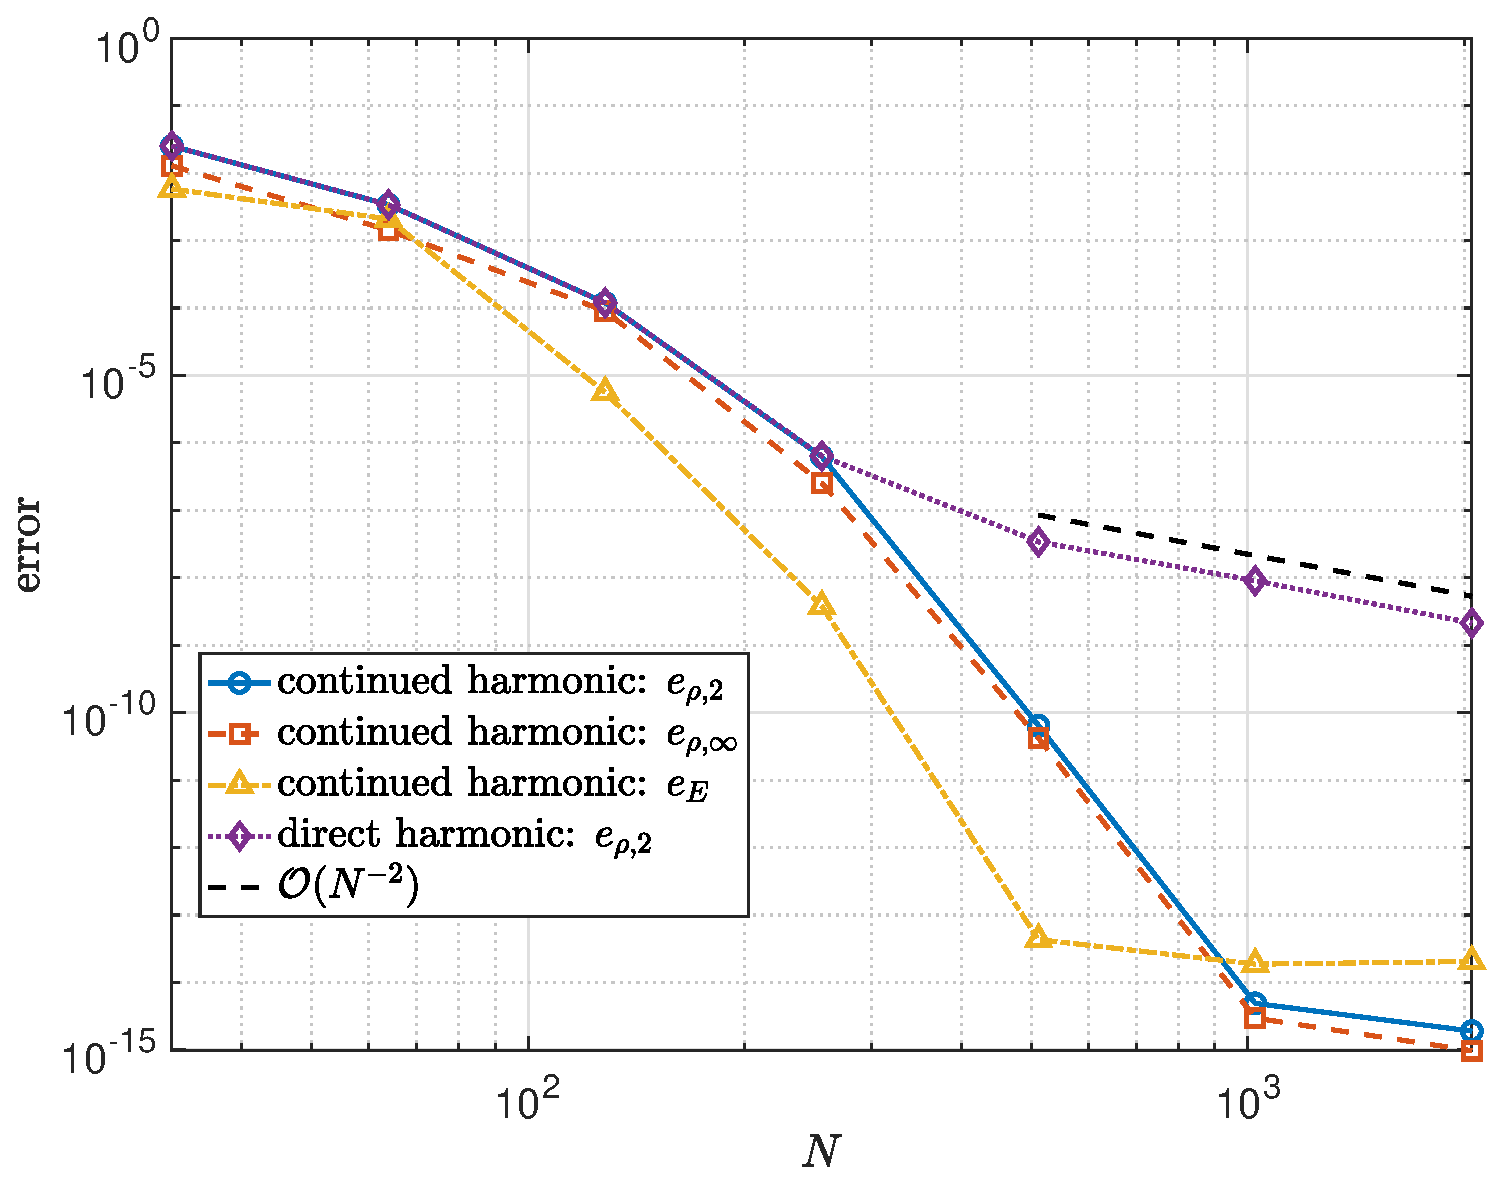
\includegraphics[width=0.7\textwidth]
{figs/mesh_convergence_1d_spatial_error.eps}
\caption{
Fourier spatial convergence for the fixed regularized problem.
The continued harmonic potential yields rapid decay of the state and
energy errors, while the direct periodic treatment of the harmonic
potential develops a high-resolution algebraic error floor.
}
\label{fig:mesh-convergence}
\end{figure}


% ------------------------------------------------------------
\subsection{Regularization effects}
\label{subsec:num-regularization}
% ------------------------------------------------------------

The regularized model contains two parameters associated with the
kinetic and potential terms. We first examine the effect of the
potential regularization parameter $\sig$ at fixed $\eps$, including
its influence on Fourier resolution. We then compare different
regularizations of the density kinetic term as $\eps\to0$.

\paragraph{Potential regularization.}

We fix $\eps=10^{-2}$, $L=32$, and $N=4096$, and take
$\sig=\eps^p$ with $p=1,2,3,4$. Let $\rho_{\eps,\sig}$ denote the
minimizer with the regularized potential, and let $\rho_{\eps,0}$
denote the minimizer obtained with the same kinetic regularization but
the original linear potential. To quantify the perturbation introduced
by $p_\sig$, we define
\begin{equation}
\label{eq:num-potential-bias}
\begin{aligned}
B_E(\sig)
&=
E_{\eps,0}(\rho_{\eps,\sig})
-
E_{\eps,0}(\rho_{\eps,0}),
\\
B_\rho(\sig)
&=
\norm{
\rho_{\eps,\sig}-\rho_{\eps,0}
}_{L^2(D_L)}.
\end{aligned}
\end{equation}
Here $E_{\eps,0}$ denotes the energy with the same denominator
$r_\eps$ and the original potential contribution $V\rho$.



\begin{table}[t]
\centering
\small
\caption{
Effect of the potential regularization scale at
$\eps=10^{-2}$, $L=32$, and $N=4096$.
The quantities $B_E$ and $B_\rho$ are defined in
\eqref{eq:num-potential-bias}.
}
\label{tab:sigma-sweep}
\begin{tabular}{cccc}
\toprule
$\sig$
&
$B_E(\sig)$
&
$B_\rho(\sig)$
&
$\min\rho$
\\
\midrule
$10^{-2}$
& $1.776\times10^{0}$
& $2.548\times10^{-2}$
& $6.449\times10^{-5}$
\\
$10^{-4}$
& $1.849\times10^{-2}$
& $2.900\times10^{-4}$
& $6.740\times10^{-7}$
\\
$10^{-6}$
& $1.849\times10^{-4}$
& $2.719\times10^{-6}$
& $6.743\times10^{-9}$
\\
$10^{-8}$
& $1.849\times10^{-6}$
& $1.993\times10^{-8}$
& $6.744\times10^{-11}$
\\
\bottomrule
\end{tabular}
\end{table}

Table~\ref{tab:sigma-sweep} shows that both perturbations decrease
approximately linearly with $\sig$ over the tested range. The minimum
density exhibits the same scaling for small $\sig$, indicating that
the positive low-density background introduced by the potential
regularization vanishes together with $\sig$.

Reducing $\sig$ also makes the regularized low-density transition
sharper. Indeed,
\[
p_\sig'(\rho)
=
\frac{\rho}{\sqrt{\rho^2+\sig^2}}
\]
is close to one where $\rho\gg\sig$ and approaches zero where
$\rho\ll\sig$. As $\sig$ decreases, the transition between these two
regimes becomes increasingly sharp. This behavior is illustrated in
Fig.~\ref{fig:regularization-sigma}.

\begin{figure}[t]
\centering
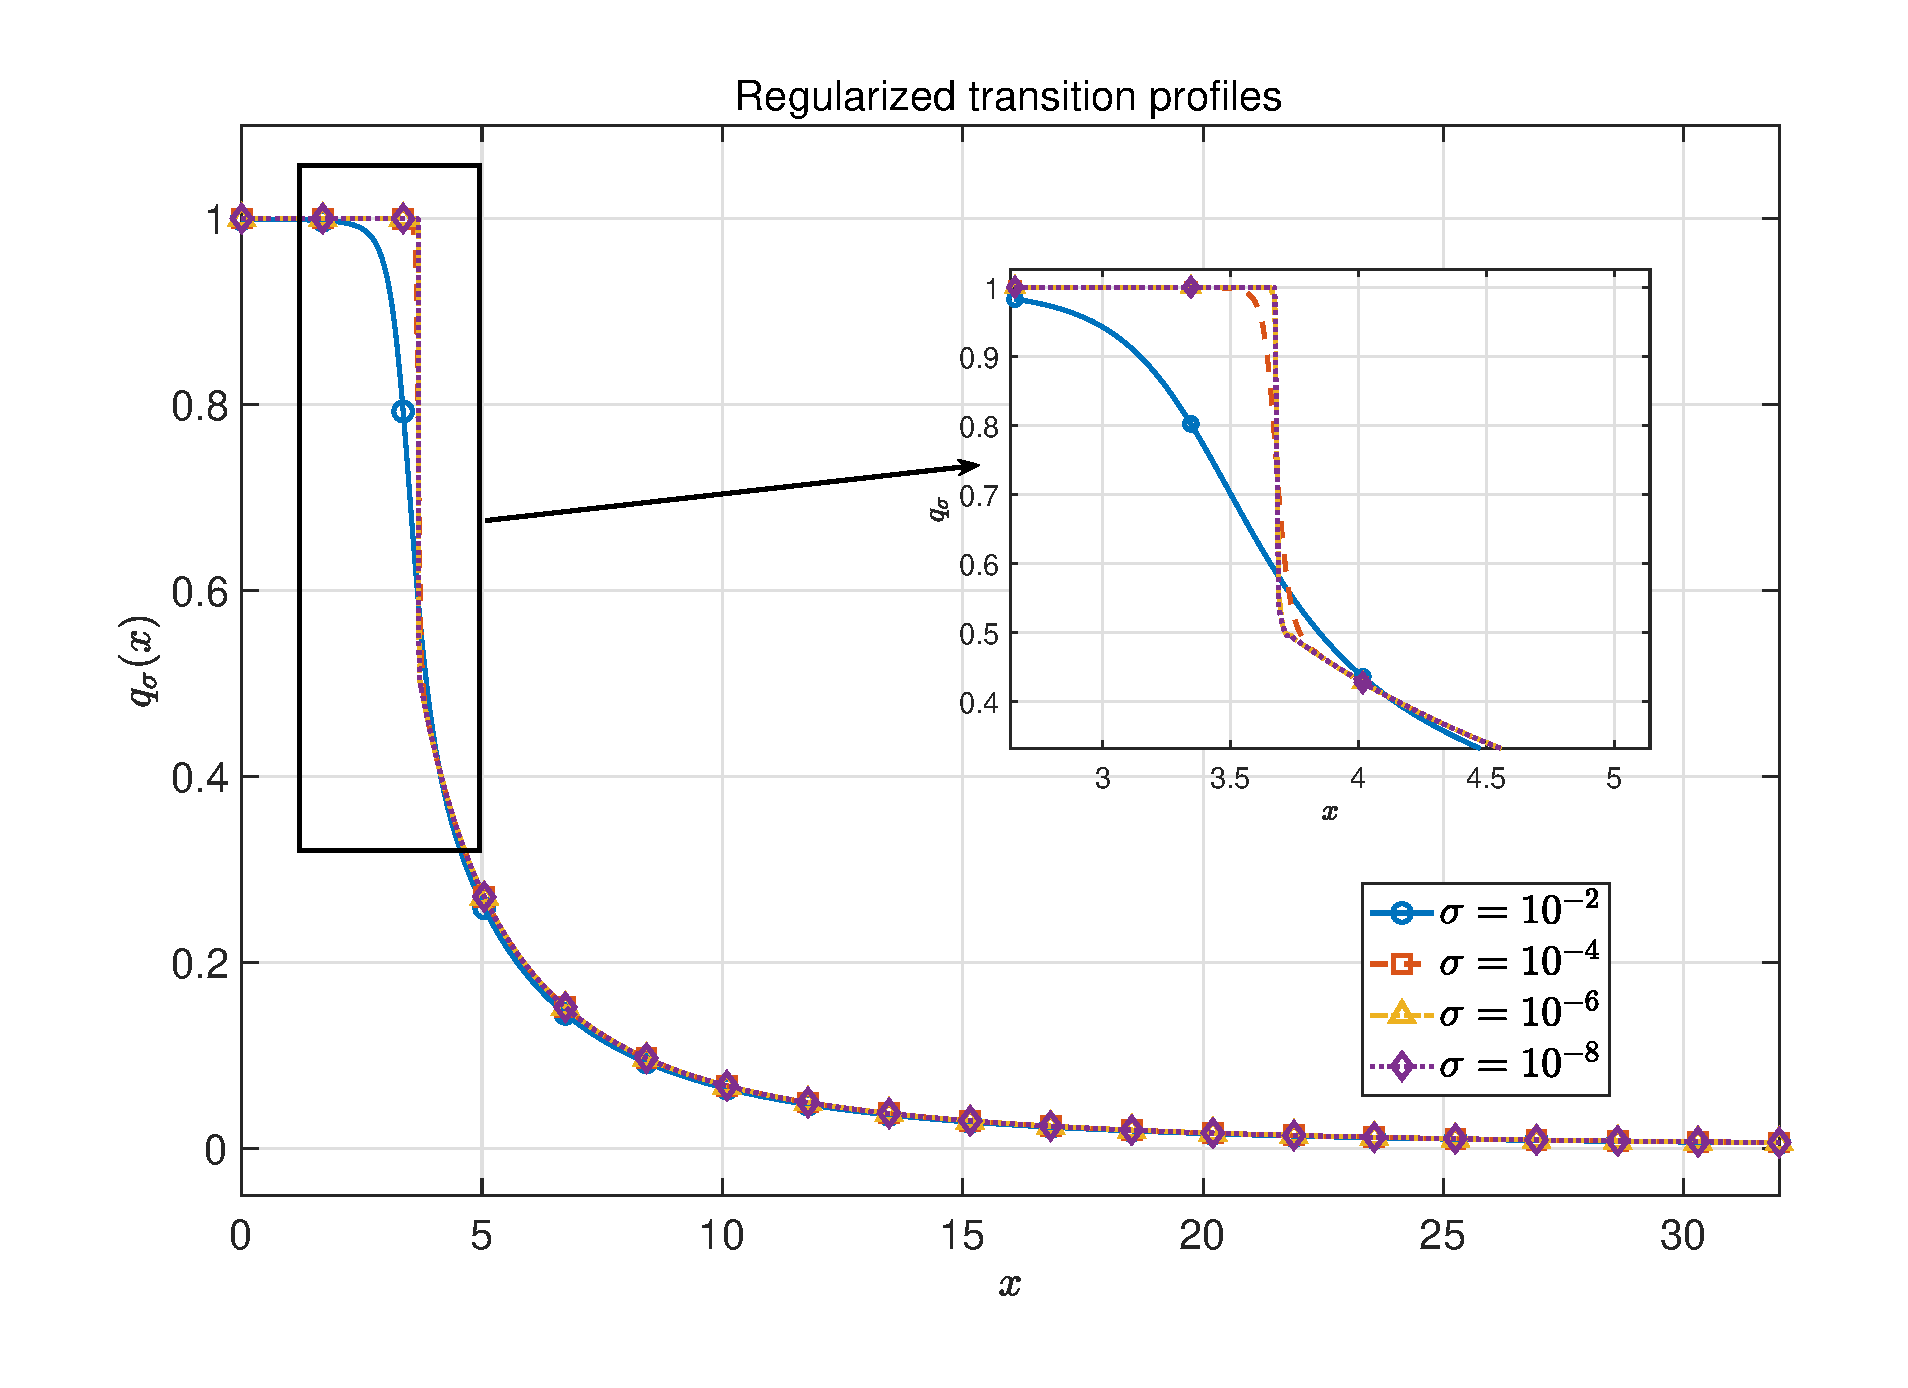
\includegraphics[width=0.70\textwidth]
{figs/regularization_sigma_L32_transition.eps}
\caption{
Transition profiles induced by the potential regularization.
As $\sig$ decreases, the transition between the bulk and low-density
regions becomes sharper. The inset enlarges the principal transition
region. All computations use $\eps=10^{-2}$, $L=32$, and $N=4096$.
}
\label{fig:regularization-sigma}
\end{figure}


To examine the resulting effect on Fourier resolution, we repeat the
mesh refinement for
$\sig=10^{-2},10^{-4},10^{-6}$, while keeping
$\eps=10^{-2}$ and $L=32$. We use the same $C^\infty$-continued
harmonic potential as in Subsection~\ref{subsec:num-mesh}, and measure
the errors relative to an $N_{\rm ref}=65536$ comparison state.
Figure~\ref{fig:sigma-accuracy} shows the resulting energy and state
errors.

\begin{figure}[t]
\centering
\includegraphics[width=0.48\textwidth]
{figs/sigma_effect_energy_error_1d.eps}
\includegraphics[width=0.48\textwidth]
{figs/sigma_effect_state_error_1d.eps}
\caption{
Effect of the potential regularization scale on Fourier accuracy.
The left panel shows the energy error and the right panel shows the
total spectral $L^2$ state error. Each curve refines a fixed-$\sig$
problem with $\eps=10^{-2}$, $L=32$, and the harmonic-core
$C^\infty$ far-field continuation, relative to the
$N_{\rm ref}=65536$ comparison state.
}
\label{fig:sigma-accuracy}
\end{figure}

For $\sig=10^{-2}$, both errors rapidly enter the spectral regime and
reach their numerical floors. As $\sig$ decreases, a longer
pre-asymptotic range appears before the rapid spectral-type decay
becomes visible. Thus a smaller $\sig$ reduces the potential
regularization error but simultaneously sharpens the transition and
requires a finer Fourier mesh. This bias--resolution tradeoff explains
why the spatial-convergence experiment in
Subsection~\ref{subsec:num-mesh} keeps the regularization parameters
fixed rather than sending them to zero together with the mesh size.


\paragraph{Regularization of the kinetic term.}

We next isolate the effect of the kinetic regularization by fixing the
potential regularization and the spatial discretization. We compare
the shifted denominator \eqref{eq:shift-denominator} with the
piecewise $C^1$ and $C^2$ denominators in
\eqref{eq:piecewise-regularization-family}. Throughout this test, we
take $\sig=10^{-2}$, $L=32$, and $N=512$, and use the same
$C^\infty$-continued harmonic potential. The tested values are
$\eps=10^{-1},5\times10^{-2},2\times10^{-2},10^{-2},
5\times10^{-3},2\times10^{-3},10^{-3}$.

A common reference state $\rho_{\rm ref}$ is computed with the shifted
denominator at $\eps_{\rm ref}=10^{-5}$. To compare the three
regularizations on the same basis, we measure the state error and
evaluate the energy error with the common unregularized kinetic
denominator $r_0(\rho)=\rho$:
\begin{equation}
\label{eq:kinetic-reg-errors}
\begin{aligned}
e_\rho(\eps)
&=
\norm{\rho_\eps-\rho_{\rm ref}}_{L^2(D_L)},
\\
e_E(\eps)
&=
\abs{
E_{0,\sig}(\rho_\eps)
-
E_{0,\sig}(\rho_{\rm ref})
}.
\end{aligned}
\end{equation}
Here $E_{0,\sig}$ denotes the energy with the original kinetic
denominator $r_0(s)=s$ and the fixed potential regularization
$p_\sig$. Thus the energy comparison measures the effect of the
computed states rather than the direct change of the regularized
energy functional.

\begin{figure}[t]
\centering
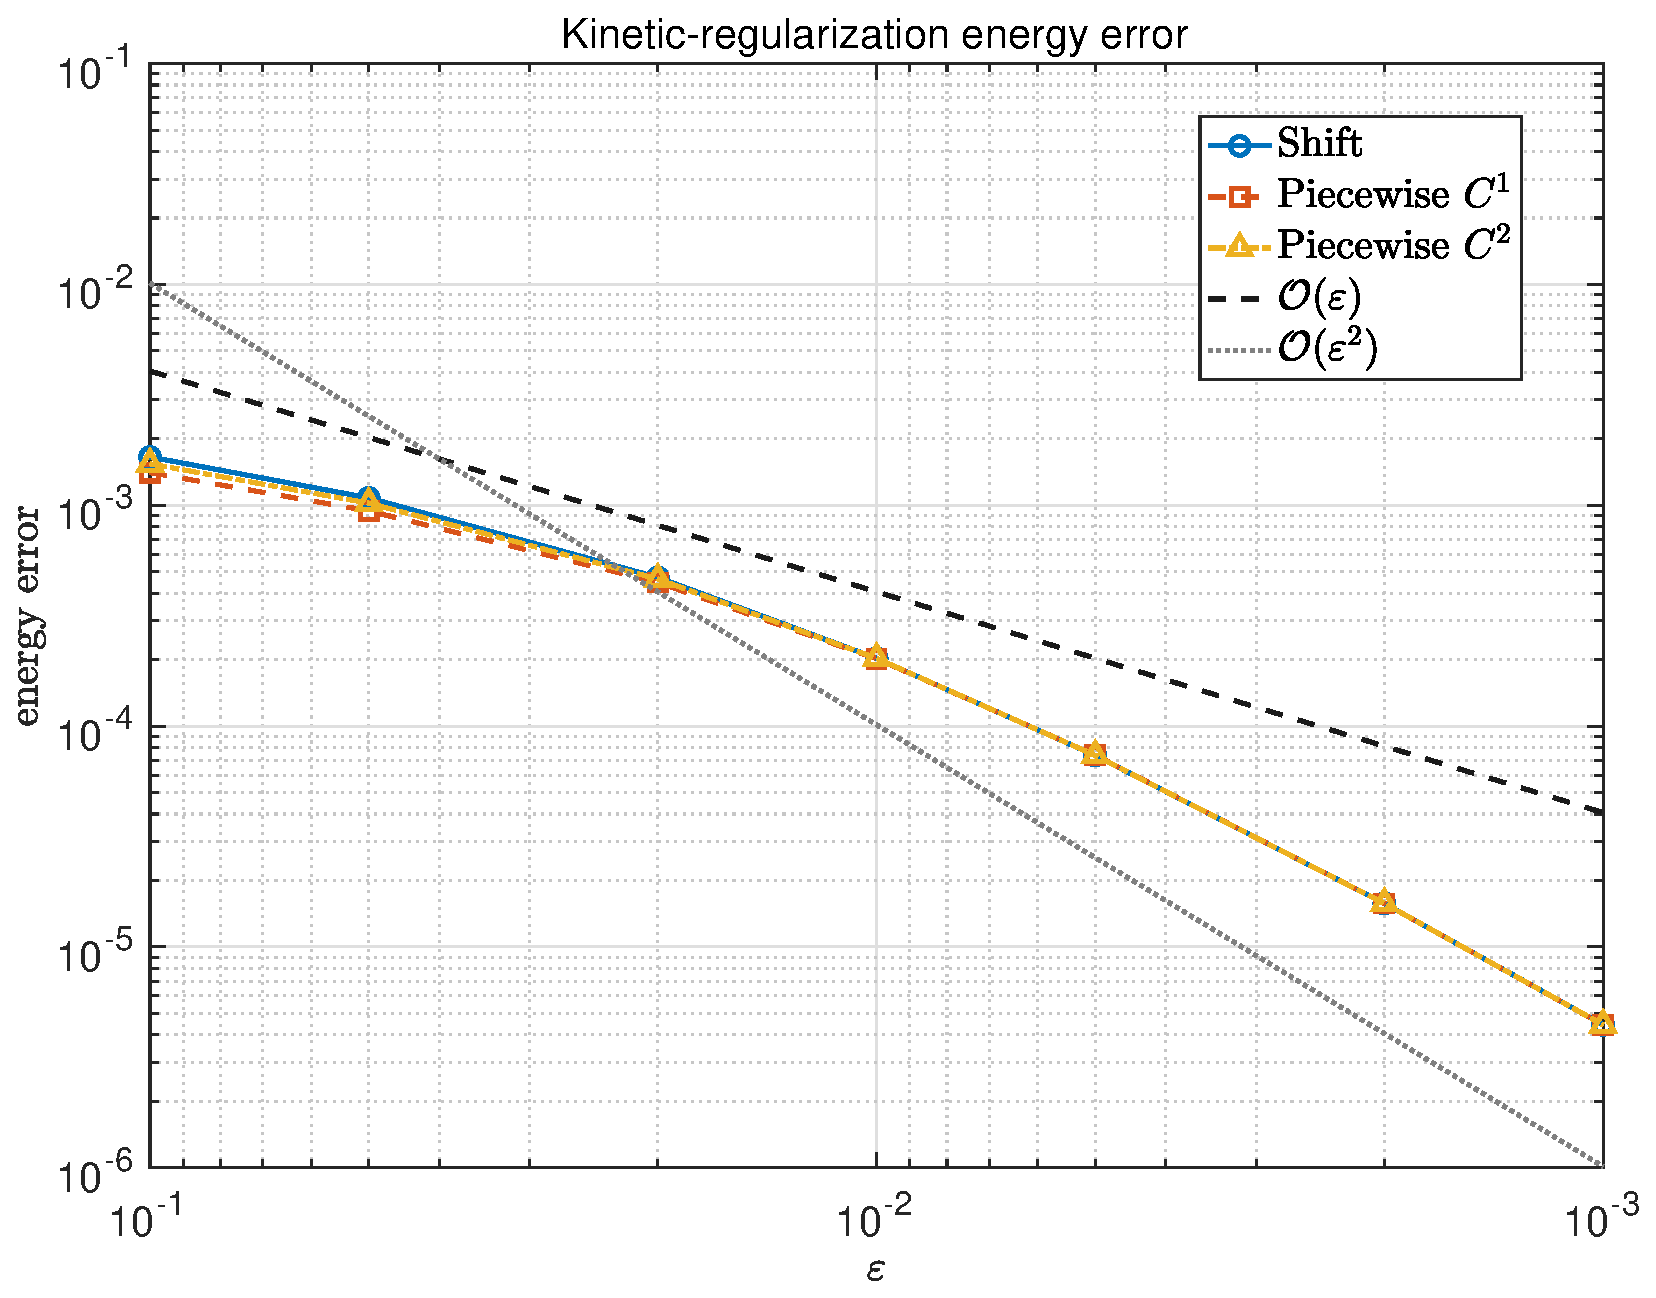
\includegraphics[width=0.48\textwidth]
{figs/kinetic_regularization_energy_error.eps}
\hfill
\includegraphics[width=0.48\textwidth]
{figs/kinetic_regularization_state_error.eps}
\caption{
Effect of the kinetic regularization. The shifted and piecewise
$C^1/C^2$ denominators are compared using the same potential
regularization, Fourier resolution, and reference state. The left
panel shows the $L^2$ state error and the right panel shows the energy
error evaluated with the common unregularized kinetic denominator
$r_0(s)=s$. The dashed and dotted lines indicate first- and
second-order slopes, respectively.
}
\label{fig:kinetic-regularization}
\end{figure}

Figure~\ref{fig:kinetic-regularization} shows that the three
regularizations have essentially the same asymptotic behavior as
$\eps$ decreases. 
The common-functional energy error approaches second order whereas the state error is approximately first order.
The piecewise $C^1$ denominator gives a modest reduction in error for
the larger values of $\eps$, but neither piecewise regularization
shows a clear asymptotic rate advantage over the shifted denominator.
%In all cases, the final projected-gradient residual is well below the
%reported regularization errors.

% ------------------------------------------------------------
\subsection{Solver performance}
\label{subsec:num-solver}
% ------------------------------------------------------------

We next examine the computational performance of the two-stage
optimization strategy. Throughout this subsection, we use the shifted
denominator $r_\eps(\rho)=\rho+\eps$. We first illustrate the
respective roles of FISTA and the Newton--PCG refinement, and then
examine how the two regularization scales affect the computational
cost.

\paragraph{FISTA and Newton refinement.}

We consider the representative case
$\eps=10^{-2}$, $\sig=10^{-4}$, $L=32$, and $N=4096$.
A common FISTA iteration is first run until the switching criterion is
met. From the resulting state, one branch continues with FISTA, while
the other proceeds with the Newton--PCG refinement. The two strategies
therefore share exactly the same first-order history up to the switch.

Since FISTA and Newton steps have different computational costs,
Fig.~\ref{fig:solver-performance} reports the convergence histories
against cumulative wall-clock time. The common prefix uses a single
time history, after which the incremental time of each branch is added
to the common switch time. The left panel shows the energy error
relative to the final two-stage solution, while the right panel shows
the projected-gradient residual. The marker denotes the switch to the
Newton--PCG refinement.

\begin{figure}[t]
\centering
\includegraphics[width=0.48\textwidth]
{figs/solver_energy_history_shared_prefix.eps}
\hfill
\includegraphics[width=0.48\textwidth]
{figs/solver_residual_history_shared_prefix.eps}
\caption{
Convergence histories for continued FISTA and the two-stage
FISTA--Newton strategy with
$\eps=10^{-2}$, $\sig=10^{-4}$, $L=32$, and $N=4096$.
The left panel shows the energy error relative to the final two-stage
solution, and the right panel shows the projected-gradient residual.
The two curves share exactly the same FISTA history up to the marker,
which denotes the switch to the Newton--PCG refinement; thereafter one
branch continues FISTA and the other uses Newton--PCG.
}
\label{fig:solver-performance}
\end{figure}

At the switch, after $3025$ FISTA iterations and $106.31$ s, the
energy has already reached its numerical plateau,
whereas the projected-gradient residual remains appreciably larger
than the final tolerance. Continued FISTA reduces this residual only
slowly, while the Newton--PCG refinement rapidly reaches high-accuracy
stationarity. In the shared-prefix experiment, the two-stage method
reaches a projected-gradient residual of $3.11\times10^{-11}$ at a
cumulative time of $107.02$ s. Continued FISTA has a residual of
$3.25\times10^{-8}$ after $50000$ iterations and $1790.63$ s.
The comparison therefore highlights the complementary roles of the
two stages: FISTA provides the main energy minimization, while
Newton--PCG efficiently resolves the remaining stationarity error.


\paragraph{Dependence on the regularization scales.}

We next examine how the computational cost changes as the
regularization parameters decrease. To isolate the two effects, we
first vary $\eps$ at fixed $\sig=10^{-2}$ and then vary $\sig$ at
fixed $\eps=10^{-2}$. In all cases,
$r_\eps(\rho)=\rho+\eps$.

All runs use the same Fourier resolution $N=4096$, initial density,
and solver parameters. Thus the comparison reflects changes in the
conditioning of the regularized problem rather than changes in the
number of Fourier degrees of freedom. The results are summarized in
Table~\ref{tab:solver-regularization-cost}.
Here wall-clock time comprises the production FISTA stage and the
Newton--PCG KKT refinement, including their standard convergence
diagnostics, but excludes problem construction, initialization, file
I/O, plotting, and experiment-specific postprocessing.

\begin{table}[t]
\centering
\caption{
Computational cost of the two-stage solver for different
regularization scales. The shifted denominator
$r_\eps(\rho)=\rho+\eps$ is used in all cases, with the same
initialization, Fourier resolution $N=4096$, and solver parameters.
``FISTA'' and ``Newton'' denote the iteration counts in the two
stages, and ``PCG'' is the accumulated number of inner PCG
iterations. The last column reports the final projected-gradient
residual $\|\mathcal G_{\tau_r}(\rho)\|_h$ \eqref{eq:pg-map}. The asterisk indicates that the FISTA stage reached the
prescribed iteration limit.
}
\label{tab:solver-regularization-cost}
\begin{tabular}{ccccccc}
\toprule
$\eps$ & $\sig$
& FISTA & Newton & PCG
& time (s) & $\|\mathcal G_{\tau_r}(\rho)\|_h$ \\
\midrule
$10^{-2}$ & $10^{-2}$ & 3422 & 8 & 125 & 93.50 & $5.04\times10^{-11}$ \\
$10^{-3}$ & $10^{-2}$ & 9042 & 10 & 187 & 201.64 & $2.54\times10^{-10}$ \\
$10^{-4}$ & $10^{-2}$ & $20000^*$ & 14 & 280 & 519.77 & $1.15\times10^{-9}$ \\
\midrule
$10^{-2}$ & $10^{-3}$ & 2992 & 10 & 186 & 99.28 & $3.93\times10^{-11}$ \\
$10^{-2}$ & $10^{-4}$ & 3025 & 18 & 341 & 107.02 & $3.11\times10^{-11}$
\\
\bottomrule
\end{tabular}
\end{table}

At fixed $\sig=10^{-2}$, decreasing $\eps$ makes the regularized
kinetic term increasingly stiff in low-density regions. This is
reflected in the larger FISTA iteration counts and total solution
times in Table~\ref{tab:solver-regularization-cost}. The smallest
$\eps$ case reaches the prescribed FISTA iteration limit and has a
somewhat larger final residual than the other runs.

By contrast, decreasing $\sig$ at fixed $\eps=10^{-2}$ does not
produce the same monotone increase in total cost over the tested
range. Although a smaller $\sig$ sharpens the potential transition
and changes the cost of the proximal and Newton stages, the
potential-proximal splitting keeps the large curvature
$p_\sig''(0)=1/\sig$ outside the smooth FISTA gradient. This behavior
is consistent with the motivation for the splitting in
Subsection~\ref{subsec:potential_FISTA}.


% ------------------------------------------------------------
\subsection{Two-dimensional examples}
\label{subsec:num-2d}
% ------------------------------------------------------------

We conclude the numerical study with two two-dimensional examples to
illustrate the applicability of the method to more general trapping
potentials. The effects of the Fourier resolution, regularization
parameters, and optimization accuracy have already been examined in
the preceding subsections, so no additional convergence study is
performed here.

Throughout this subsection, we use the shifted denominator
$r_\eps(\rho)=\rho+\eps$, the potential regularization $p_\sig$, and
the parameters
$\beta=\delta=10$, $\eps=10^{-2}$, and $\sig=10^{-4}$.
The computations are carried out on the periodic box
$[-16,16]^2$ with $N_x=N_y=512$ Fourier collocation points.
As in the one-dimensional experiments, the harmonic part of the
potential is left unchanged in the central region and smoothly
continued to a constant near the periodic boundary.

We first consider the anisotropic harmonic trap
\begin{equation}
\label{eq:2d-anisotropic-harmonic}
V_{\rm ah}(x,y)
=
\frac12
\left(
\gamma_x^2x^2+\gamma_y^2y^2
\right),
\qquad
\gamma_x=1,
\quad
\gamma_y=2.
\end{equation}
The resulting ground-state density is shown in the left panel of
Fig.~\ref{fig:two-dimensional-examples}. The stronger confinement in
the $y$-direction produces the expected anisotropic density profile.

As a second example, we add a square optical lattice to the same
harmonic confinement,
\begin{equation}
\label{eq:2d-optical-lattice}
V_{\rm ol}(x,y)
=
V_{\rm ah}(x,y)
+
V_0
\left[
\sin^2(kx)+\sin^2(ky)
\right],
\end{equation}
with $V_0=5$ and $k=\pi/2$. The additional periodic structure creates
multiple local wells and leads to the more structured density profile
shown in the right panel of
Fig.~\ref{fig:two-dimensional-examples}. This example illustrates
that the potential-proximal formulation is not restricted to a
single-well trapping potential.

\begin{figure}[htbp]
\centering
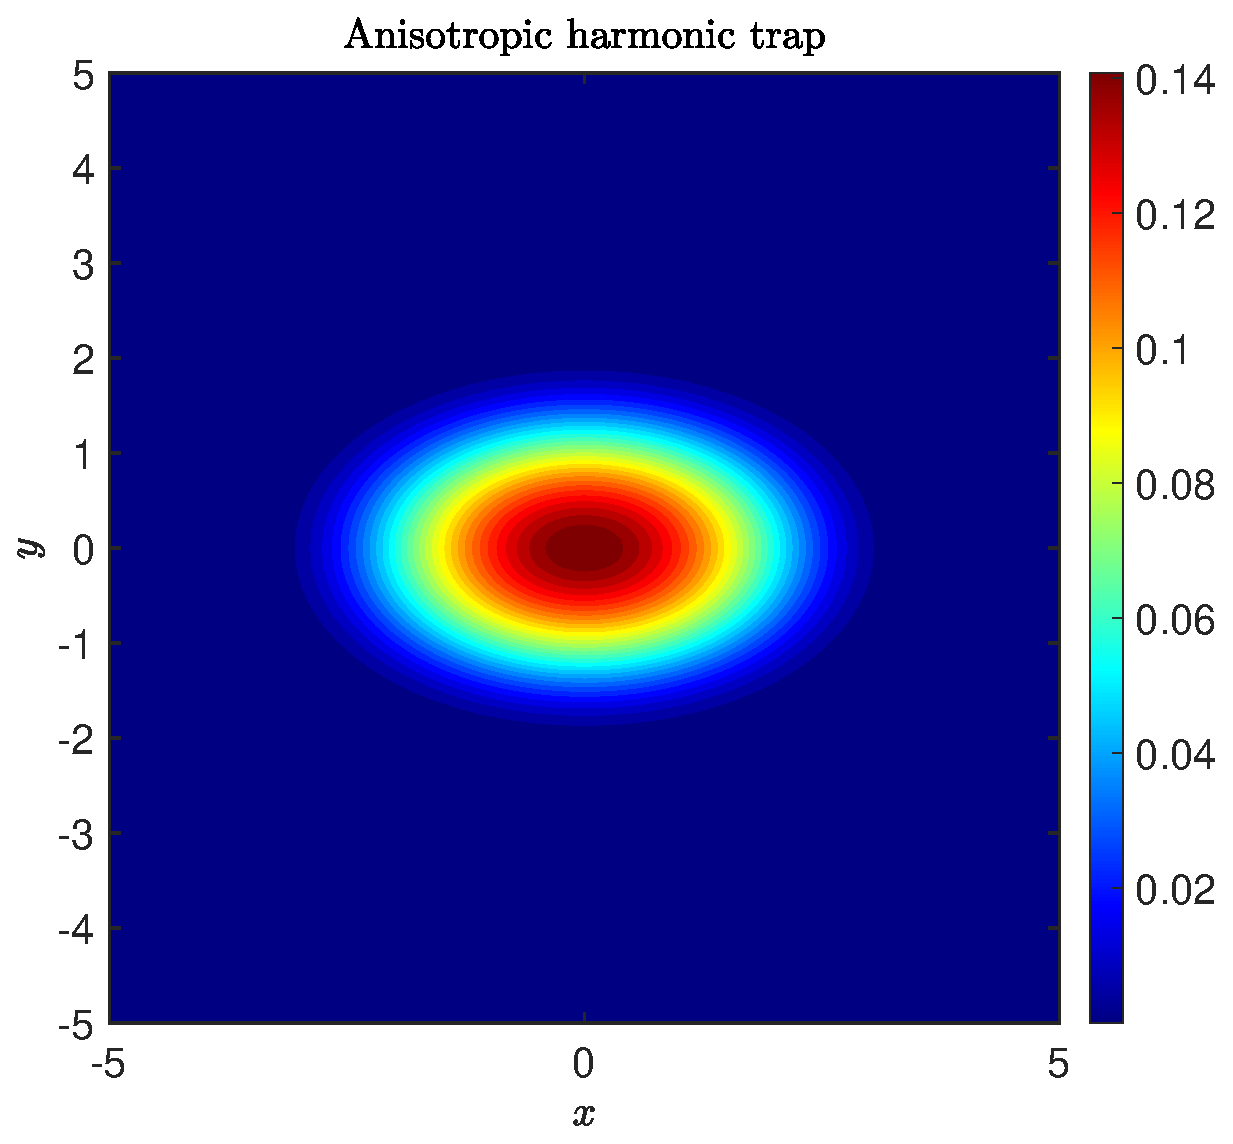
\includegraphics[width=0.48\textwidth]
{figs/ground_state_2d_anisotropic_harmonic.eps}
\hfill
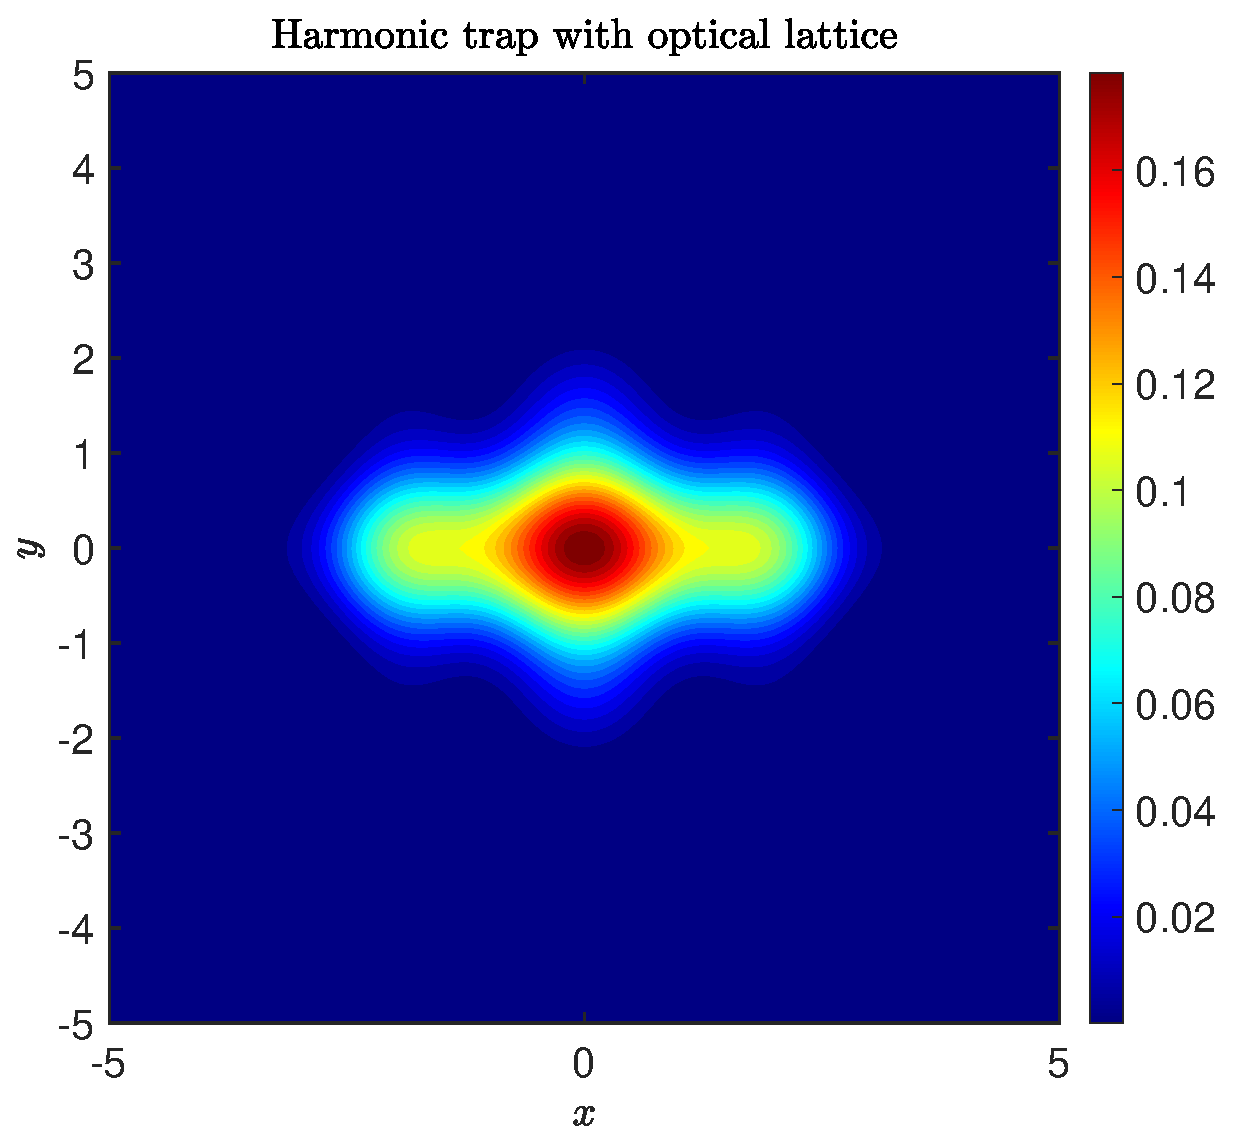
\includegraphics[width=0.48\textwidth]
{figs/ground_state_2d_optical_lattice.eps}
\caption{
Two-dimensional ground-state densities computed on $[-16,16]^2$
with $N_x=N_y=512$, with the central region shown.
The left panel corresponds to the anisotropic harmonic trap
\eqref{eq:2d-anisotropic-harmonic}, while the right panel includes
the square optical lattice \eqref{eq:2d-optical-lattice}.
Both computations use $\eps=10^{-2}$, $\sig=10^{-4}$, and
$\beta=\delta=10$.
}
\label{fig:two-dimensional-examples}
\end{figure}


% ============================================================
\section{Conclusion}
\label{sec:summary}
% ============================================================

We have developed a convex Fourier pseudospectral method for computing
ground states of Bose--Einstein condensates with higher-order
interactions in the density formulation. The singular kinetic term and
the vacuum behavior of the potential are treated by two compatible
convex regularizations, whose fixed-box energies $\Gamma$-converge to
the original density energy as the regularization parameters vanish.

The resulting discretization preserves mass and nodal positivity.
A potential-proximal FISTA iteration provides the main minimization,
followed by a Newton--PCG refinement for high-accuracy stationarity.
Numerical experiments demonstrate spectral-type convergence for fixed
smooth regularized problems and reveal the bias--resolution tradeoff
associated with the potential regularization. A joint analysis of the
box, Fourier, and regularization limits remains for future work.
% ============================================================
\appendix

% ============================================================
\section{KKT system for the positive conservative projection}
\label{app:projection-kkt}
% ============================================================

For completeness, consider the nodal projection
\[
\min_y
\frac12\norm{y-z}_h^2
\quad
\text{subject to}
\quad
y\ge0,
\qquad
h\bm1^Ty=1.
\]
Its KKT conditions are
\[
y-z-\lambda\bm1-\mu=0,
\qquad
y\ge0,
\qquad
\mu\ge0,
\qquad
y_j\mu_j=0.
\]
It follows that
\[
y_j=\max\{z_j+\lambda,0\},
\]
where $\lambda$ is determined by the monotone mass equation
\[
h\sum_j\max\{z_j+\lambda,0\}=1.
\]
This gives the scalar characterization of the positive
mass-conservative projection used in Section~\ref{sec:ps}.


% ============================================================
\section{Newton--PCG implementation}
\label{app:newton-implementation}
% ============================================================

We record the Hessian action and finite-difference preconditioner used
in the Newton--PCG refinement. For compactness, let
\[
a=r_\eps(\rho),
\qquad
a'=r_\eps'(\rho),
\qquad
a''=r_\eps''(\rho),
\qquad
q=D_N\rho,
\qquad
\dot q=D_N\eta.
\]
At points where $r_\eps$ is twice differentiable, the Hessian action
of the regularized kinetic term is
\begin{align}
\label{eq:hessian-action}
H_{\rm kin}(\rho)[\eta]
={}&
\frac14D_N^T
\left[
\frac{\dot q}{a}
-
\frac{q\,a'}{a^2}\eta
\right]
-
\frac18
\left[
2q\dot q\,\frac{a'}{a^2}
+
q^2
\left(
\frac{a''}{a^2}
-
\frac{2(a')^2}{a^3}
\right)\eta
\right].
\end{align}
The full Hessian action is
\begin{equation}
\label{eq:full-hessian-action}
H(\rho)[\eta]
=
H_{\rm kin}(\rho)[\eta]
+
Vp_\sig''(\rho)\eta
+
\beta\eta
+
\delta D_N^TD_N\eta.
\end{equation}

For the PCG preconditioner, let $D_{\rm FD}$ denote the periodic
forward-difference operator and define
\[
B_{\rm FD}
=
D_{\rm FD}
-
\operatorname{diag}\left(\frac{q\,a'}{a}\right),
\qquad
W
=
\operatorname{diag}\left(\frac1{4a}\right),
\qquad
R_{\rm kin}
=
\operatorname{diag}\left(
-\frac{q^2a''}{8a^2}
\right).
\]
We use the sparse approximation
\begin{equation}
\label{eq:fd-preconditioner}
P_{\rm FD}
=
B_{\rm FD}^TWB_{\rm FD}
+
R_{\rm kin}
+
\delta D_{\rm FD}^TD_{\rm FD}
+
\operatorname{diag}\bigl(\beta+Vp_\sig''(\rho)\bigr).
\end{equation}
In the strongly convex regime, $P_{\rm FD}$ is symmetric positive
definite. It is used only as a preconditioner; the discrete energy,
gradient, and Hessian action remain Fourier pseudospectral.

\begin{thebibliography}{99}

\bibitem{AltmannHenningPeterseim2021}
R.~Altmann, P.~Henning, and D.~Peterseim,
\newblock The J-method for the Gross--Pitaevskii eigenvalue problem,
\newblock \emph{Numer. Math.}, 148 (2021), pp.~575--610.

\bibitem{Anderson1995}
M.~H. Anderson, J.~R. Ensher, M.~R. Matthews, C.~E. Wieman,
and E.~A. Cornell,
\newblock Observation of Bose--Einstein condensation in a dilute
atomic vapor,
\newblock \emph{Science}, 269 (1995), pp.~198--201.

\bibitem{AntoineDuboscq2014}
X.~Antoine and R.~Duboscq,
\newblock Robust and efficient preconditioned Krylov spectral solvers
for computing the ground states of fast rotating and strongly
interacting Bose--Einstein condensates,
\newblock \emph{J. Comput. Phys.}, 258 (2014), pp.~509--523.

\bibitem{AntoineLevittTang2017}
X.~Antoine, A.~Levitt, and Q.~Tang,
\newblock Efficient spectral computation of the stationary states of
rotating Bose--Einstein condensates by preconditioned nonlinear
conjugate gradient methods,
\newblock \emph{J. Comput. Phys.}, 343 (2017), pp.~92--109.

\bibitem{BaoCaiReview}
W.~Bao and Y.~Cai,
\newblock Mathematical theory and numerical methods for Bose--Einstein condensation,
\newblock \emph{Kinet. Relat. Models}, 6 (2013), pp.~1--135.

\bibitem{BaoCaiRuan2019}
W.~Bao, Y.~Cai, and X.~Ruan,
\newblock Ground states of Bose--Einstein condensates with higher order interaction,
\newblock \emph{Physica D}, 386--387 (2019), pp.~38--48.

\bibitem{BaoChernLim2006}
W.~Bao, I.-L.~Chern, and F.~Y.~Lim,
\newblock Efficient and spectrally accurate numerical methods for
computing ground and first excited states in Bose--Einstein
condensates,
\newblock \emph{J. Comput. Phys.}, 219 (2006), pp.~836--854.

\bibitem{BaoDu2004}
W.~Bao and Q.~Du,
\newblock Computing the ground state solution of Bose--Einstein condensates by a
normalized gradient flow,
\newblock \emph{SIAM J. Sci. Comput.}, 25 (2004), pp.~1674--1697.

\bibitem{BaoRuan2019}
W.~Bao and X.~Ruan,
\newblock Computing ground states of Bose--Einstein condensates with higher order
interaction via a regularized density function formulation,
\newblock \emph{SIAM J. Sci. Comput.}, 41 (2019), pp.~B1284--B1309.

\bibitem{BaoTang2003}
W.~Bao and W.~Tang,
\newblock Ground-state solution of Bose--Einstein condensate by
directly minimizing the energy functional,
\newblock \emph{J. Comput. Phys.}, 187 (2003), pp.~230--254.

\bibitem{BeckTeboulle2009}
A.~Beck and M.~Teboulle,
\newblock A fast iterative shrinkage-thresholding algorithm for linear inverse problems,
\newblock \emph{SIAM J. Imaging Sci.}, 2 (2009), pp.~183--202.

\bibitem{Braides2002}
A.~Braides,
\newblock \emph{Gamma-Convergence for Beginners},
\newblock Oxford University Press, Oxford, 2002.

\bibitem{ChambolleDossal2015}
A.~Chambolle and C.~Dossal,
\newblock On the convergence of the iterates of the ``fast iterative
shrinkage/thresholding algorithm'',
\newblock \emph{J. Optim. Theory Appl.}, 166 (2015), pp.~968--982.

\bibitem{ChenLuLuZhang2024}
Z.~Chen, J.~Lu, Y.~Lu, and X.~Zhang,
\newblock On the convergence of Sobolev gradient flow for the
Gross--Pitaevskii eigenvalue problem,
\newblock \emph{SIAM J. Numer. Anal.}, 62 (2024), pp.~667--691.

\bibitem{Chin2010}
C.~Chin, R.~Grimm, P.~Julienne, and E.~Tiesinga,
\newblock Feshbach resonances in ultracold gases,
\newblock \emph{Rev. Mod. Phys.}, 82 (2010), pp.~1225--1286.

\bibitem{CollinMassignanPethick2007}
A.~Collin, P.~Massignan, and C.~J. Pethick,
\newblock Energy-dependent effective interactions for dilute
many-body systems,
\newblock \emph{Phys. Rev. A}, 75 (2007), 013615.

\bibitem{DanailaKazemi2010}
I.~Danaila and P.~Kazemi,
\newblock A new Sobolev gradient method for direct minimization of the
Gross--Pitaevskii energy with rotation,
\newblock \emph{SIAM J. Sci. Comput.}, 32 (2010), pp.~2447--2467.

\bibitem{DanailaProtas2017}
I.~Danaila and B.~Protas,
\newblock Computation of ground states of the Gross--Pitaevskii
functional via Riemannian optimization,
\newblock \emph{SIAM J. Sci. Comput.}, 39 (2017), pp.~B1102--B1129.

\bibitem{FuWangGao2003}
H.~Fu, Y.~Wang, and B.~Gao,
\newblock Beyond the Fermi pseudopotential: A modified
Gross--Pitaevskii equation,
\newblock \emph{Phys. Rev. A}, 67 (2003), 053612.

\bibitem{HenningPeterseim2020}
P.~Henning and D.~Peterseim,
\newblock Sobolev gradient flow for the Gross--Pitaevskii eigenvalue
problem: Global convergence and computational efficiency,
\newblock \emph{SIAM J. Numer. Anal.}, 58 (2020), pp.~1744--1772.

\bibitem{Ruan2018}
X.~Ruan,
\newblock A normalized gradient flow method with
attractive--repulsive splitting for computing ground states of
Bose--Einstein condensates with higher-order interaction,
\newblock \emph{J. Comput. Phys.}, 367 (2018), pp.~374--390.

\bibitem{RuanCaiBao2016}
X.~Ruan, Y.~Cai, and W.~Bao,
\newblock Mean-field regime and Thomas--Fermi approximations of
trapped Bose--Einstein condensates with higher-order interactions in
one and two dimensions,
\newblock \emph{J. Phys. B}, 49 (2016), 125304.

\bibitem{TianCaiWuWen2020}
T.~Tian, Y.~Cai, X.~Wu, and Z.~Wen,
\newblock Ground states of spin-$F$ Bose--Einstein condensates,
\newblock \emph{SIAM J. Sci. Comput.}, 42 (2020), pp.~B983--B1013.

\bibitem{Ulbrich2011}
M.~Ulbrich,
\newblock \emph{Semismooth Newton Methods for Variational Inequalities and
Constrained Optimization Problems in Function Spaces},
\newblock SIAM, Philadelphia, 2011.

\bibitem{VekslerFishmanKetterle2014}
H.~Veksler, S.~Fishman, and W.~Ketterle,
\newblock Simple model for interactions and corrections to the
Gross--Pitaevskii equation,
\newblock \emph{Phys. Rev. A}, 90 (2014), 023620.

\bibitem{WuWenBao2017}
X.~Wu, Z.~Wen, and W.~Bao,
\newblock A regularized Newton method for computing ground states of
Bose--Einstein condensates,
\newblock \emph{J. Sci. Comput.}, 73 (2017), pp.~303--329.

\bibitem{ZinnerThogersen2009}
N.~T. Zinner and M.~Th{\o}gersen,
\newblock Stability of a Bose--Einstein condensate with higher-order
interactions near a Feshbach resonance,
\newblock \emph{Phys. Rev. A}, 80 (2009), 023607.

\end{thebibliography}

\end{document}
